\documentclass[12pt,a4paper]{uefrep}
%
% Note, if you are writing in Finnish, modify commented lines in this file and
% modify also report_app.tex if you have appendices.
%
\usepackage[english]{babel}  % If writing in Finnish, replace egnlish with finnish
\usepackage[T1]{fontenc}
\usepackage{cite,url}
\usepackage[dvips]{graphicx}
\usepackage[tbtags]{amsmath}
\usepackage{psfrag}
\usepackage{ae,aecompl}
\usepackage{color}
\usepackage{bookmark}
\usepackage[a-1b]{pdfx}
\usepackage{hyperref}
\usepackage{subcaption}
\usepackage{listings}
\usepackage{xcolor}
%\usepackage{float}
\usepackage{amsthm,amssymb}
\usepackage{tabularx}
\usepackage{longtable} % for table header multicolumn

\definecolor{dkgreen}{rgb}{0,0.6,0}
\definecolor{gray}{rgb}{0.5,0.5,0.5}
\definecolor{mauve}{rgb}{0.58,0,0.82}

\lstset{frame=tb,
  language=Python,
  aboveskip=3mm,
  belowskip=3mm,
  showstringspaces=false,
  columns=flexible,
  basicstyle=\footnotesize,
  numbers=none,
  numberstyle=\tiny\color{gray},
  keywordstyle=\color{blue},
  commentstyle=\color{dkgreen},
  stringstyle=\color{mauve},
  breaklines=true,
  breakatwhitespace=true,
  tabsize=3
}


% LET TESTING







\hypersetup{colorlinks=true,linkcolor=blue,citecolor=red,urlcolor=cyan,breaklinks=true}
%
%
\pagestyle{plain}
\bibliographystyle{uefunsrt}
\setlength{\textheight}{20.7cm}
\setlength{\textwidth}{15.0cm}
\setlength{\hoffset}{-2mm}  % Because the location of left margin depends on the printer, adjust this so that the left margin is 32 mm.
%\setlenght{\voffset}{2mm} % If necessary, adjust the top margin to 45 mm with this parameter.
%
\renewcommand{\baselinestretch}{1.2}
\newcommand{\BibTeX}{{\textrm B\kern-.05em{\textsc i\kern-.025em b}\kern-.08em
    T\kern-.1667em\lower.7ex\hbox{E}\kern-.125emX}}
\newcommand{\sep}{;~}

\newenvironment{conditions}
  {\par\vspace{\abovedisplayskip}\noindent\begin{tabular}{>{$}l<{$} @{${}={}$} l}}
  {\end{tabular}\par\vspace{\belowdisplayskip}}




\usepackage{floatrow}
% Table float box with bottom caption, box width adjusted to content
\newfloatcommand{capbtabbox}{table}[][\FBwidth]

\usepackage[font=small,labelfont=bf,tableposition=top]{caption}

\DeclareCaptionLabelFormat{andtable}{#1~#2  \&  \tablename~\thetable}





\begin{document}


%% LET TEST

\makeatletter 
\let\c@table\c@figure
\let\c@lstlisting\c@figure
\makeatother


%
\pagenumbering{roman}
%
%%% Edit properly, pay special attention to names and dates.
%
\thispagestyle{empty}
%
%\\[1.5cm]
%
{\centering
%
{\huge\textbf{Estimating installation parameters of photovoltaic systems in northern latitudes by mathematical model fitting 
%\footnote{%
%\color{red} Remember to read the report writing instructions!
%(report\_writing\_instructions.pdf)} % Remove this footnote after reading the writing instructions ;)
}}\\[1.5cm]
%
% If the title is long for a one line, divide it to multiple lines, and use the \\[2mm] command to 
% add 2mm space between the lines.
%
{\huge \textit{Timo Salola}}
%
\vfill
%
%%% Insert here a figure if you like or remove these lines
%
%\begin{figure}[!h]
%\centering
%\includegraphics[width=11cm]{fpfig.eps}
%\end{figure}
%\vfill
%
{%
\renewcommand{\baselinestretch}{1.0}
%
\texttt{\large MSc Thesis\\[1mm] % or BSc thesis
November 2023\\
Department of Physics and Mathematics\\
University of Eastern Finland\\%
}}}
%
% This will create the frame for the front page.
%
\setlength{\unitlength}{1mm}
\linethickness{1.5pt}
\vspace{-25cm}
\begin{picture}(170,260)(13.5,-5)
% 
% For displays these picture settings in brackets above are fine, but for paper prints, the
% frame position may require some adjustment. If needed, adjust the last two parameters 
% so that when printed the frame is 25 mm from left and 25 mm from top of the page
%
\put(-5,-40.3){\line(1,0){170}}
\put(-5,225){\line(1,0){170}}
\put(-5,-40.6){\line(0,1){265.84}}
\put(165,-40.6){\line(0,1){265.84}}
\end{picture}\\


\newpage
\include{thesis_abs}
%
\newpage                     % (Un)comment these lines depending on if you have or not have a preface
\phantomsection
\hypertarget{prefacepage}{}
\bookmark[dest=prefacepage]{Preface}
%
\section*{\prefacename}
%Write the preface here. n the preface, you may inform the reader about your motivation to write your thesis and your experiences during the writing of your thesis. You can also use the preface to help the reader get started and to thank people who have helped you with your hesis.
As someone whose interests and strenghts lie in geometry and programming, the real world problem of panel installation parameter estimation was appealing from the beginning. I would like to thank William Wandji and Juha Karhu for their insights on the effects of clouds, snows and temperature on solar PV installation data. And Luna for being the softest and purriest of cats.

\vspace{3mm}
\noindent This research was funded by the Academy of Finland, decision 350695.


\vspace{9mm}
\noindent
Helsinki, the 15th of August 2023 %
%
%%% the signature below has some artistic freedom : )
%
\vspace{11mm}
\hspace{1.6cm}\emph{Timo Salola}

\vfill















     %
%
\phantomsection
\hypertarget{contentpage}{}
\bookmark[dest=contentpage]{Contents}
\tableofcontents
%
\newpage
\setcounter{page}{0}
\pagenumbering{arabic}
%

% ############################## INCLUDES HERE
\chapter{Introduction}


This thesis examines a specific applied mathematics problem suggested by the Finnish Meteorological Institute(FMI). The goal is to solve the geographic location and panel installation angles of photovoltaic solar power installations using only the power output data. The chosen method breaks the problem of solving the geographic location and panel angles into separate algorithms. In practice, this means that the algorithms used can be less complex as they do not have to solve every unknown variable simultaneously and visualizations of individual algorithms should also be more straightforward as 2-dimensional data can be graphed with ease. Using multiple algorithms also splits the parameter space into smaller spaces, thus improving the performance of fitting algorithms. And the final benefit is the ability to focus on solving only the unknown parameters. For example, if the geolocation of a system is known and the panel installation angles are not, there is very little reason to use a model that would solve geolocation and panel angles without taking into account that some parameters are already known. 


The applications of parameter estimation algorithms would be in improving the quality of metadata in solar PV datasets. This could have implications for solar PV research but the existance of such algrithms poses some privacy and security related questions as well. Whether these research benefits and concerns are realized, depends on the accuracy, and to some extent the ease of use of the algorithms.
%If algorithms for solving geographic location and panel installation angles can be constructed, their immediate applications 


A similar study was done by N. Haghdadi et al. in 2017\cite{navid_australian_article}. The 2017 article contains results from five case studies where the standard deviation of longitude prediction errors is less than $1.5^\circ$, reaching as low as $0.08^\circ$ with case study 1-2. The standard deviation of latidude predictions is higher at less than 3.5$^\circ$ with the best result in case study 2-2 with standard deviation of 1.65$^\circ$. Azimuth and tilt predictions are reported as two separate angle error values with azimuth prediction errors reaching values between 4$^\circ$ and 27$^\circ$ and tilt 1.3$^\circ$ to 11.5$^\circ$. These forementioned results are not directly comparable to the results shown in this thesis due to different datasets, geographic location and local climate, but they provide some perspective.





%The most similar study to this that was found during literary review was done by N. Haghdadi et al. in 2017\cite{navid_australian_article}. In the 2017 paper, the resulting 
%Perhaps the most similar study was done by N. Haghdadi et al. in 2017\cite{navid_australian_article}. In Haghdadi's paper, the standard deviation and mean absolute deviation of estimated 


%for longitude are both less than 1.5$^\circ$ in the five listed case studies, reaching as low as 0.08$^\circ$ in case study 1-2. The standard deviation of latitudes is less than 3.5$^\circ$ for each case study; the panel tilt deviation is less than 11.5$^\circ$, and the azimuth is less than 27.5$^\circ$.
%Haghdadi's article uses the same method for determining the longitude, but the methods for determining the other variables are different. 

Another article of relevance written by M.K. Williams et. al. in 2012\cite{older_solar_solver_article} proposes multiple methods for determining the locations and orientations of solar PV installations. Perhaps the most interesting contribution of the 2012 article is the network approach to determining geographic location. This method relies on a grid of installations with known and accurate geolocation and installation angles. According to the authors, this networked approach works up to a 10-mile accuracy when the grid of known installations is dense around the estimated installation. This could make the network approach preferable for electric companies or institutions with large amounts of data. But as of now, it does not seem usable for FMI.


%These methods include the same longitude algorithm as Hagdadis's article\cite{navid_australian_article}, but perhaps the most interesting contribution is the network approach to determining geographic location. This earlier article relies on a grid of installations with known and accurate geolocation and installation angles. According to the authors, this networked approach works up to 10-mile accuracy when the grid of known installations is dense around the installation location. This could make the network approach preferable for electric companies or institutions with large amounts of data. But as of now, it does not seem usable for FMI.

\chapter{Installations and datasets}

\begin{figure}[h]
\centering
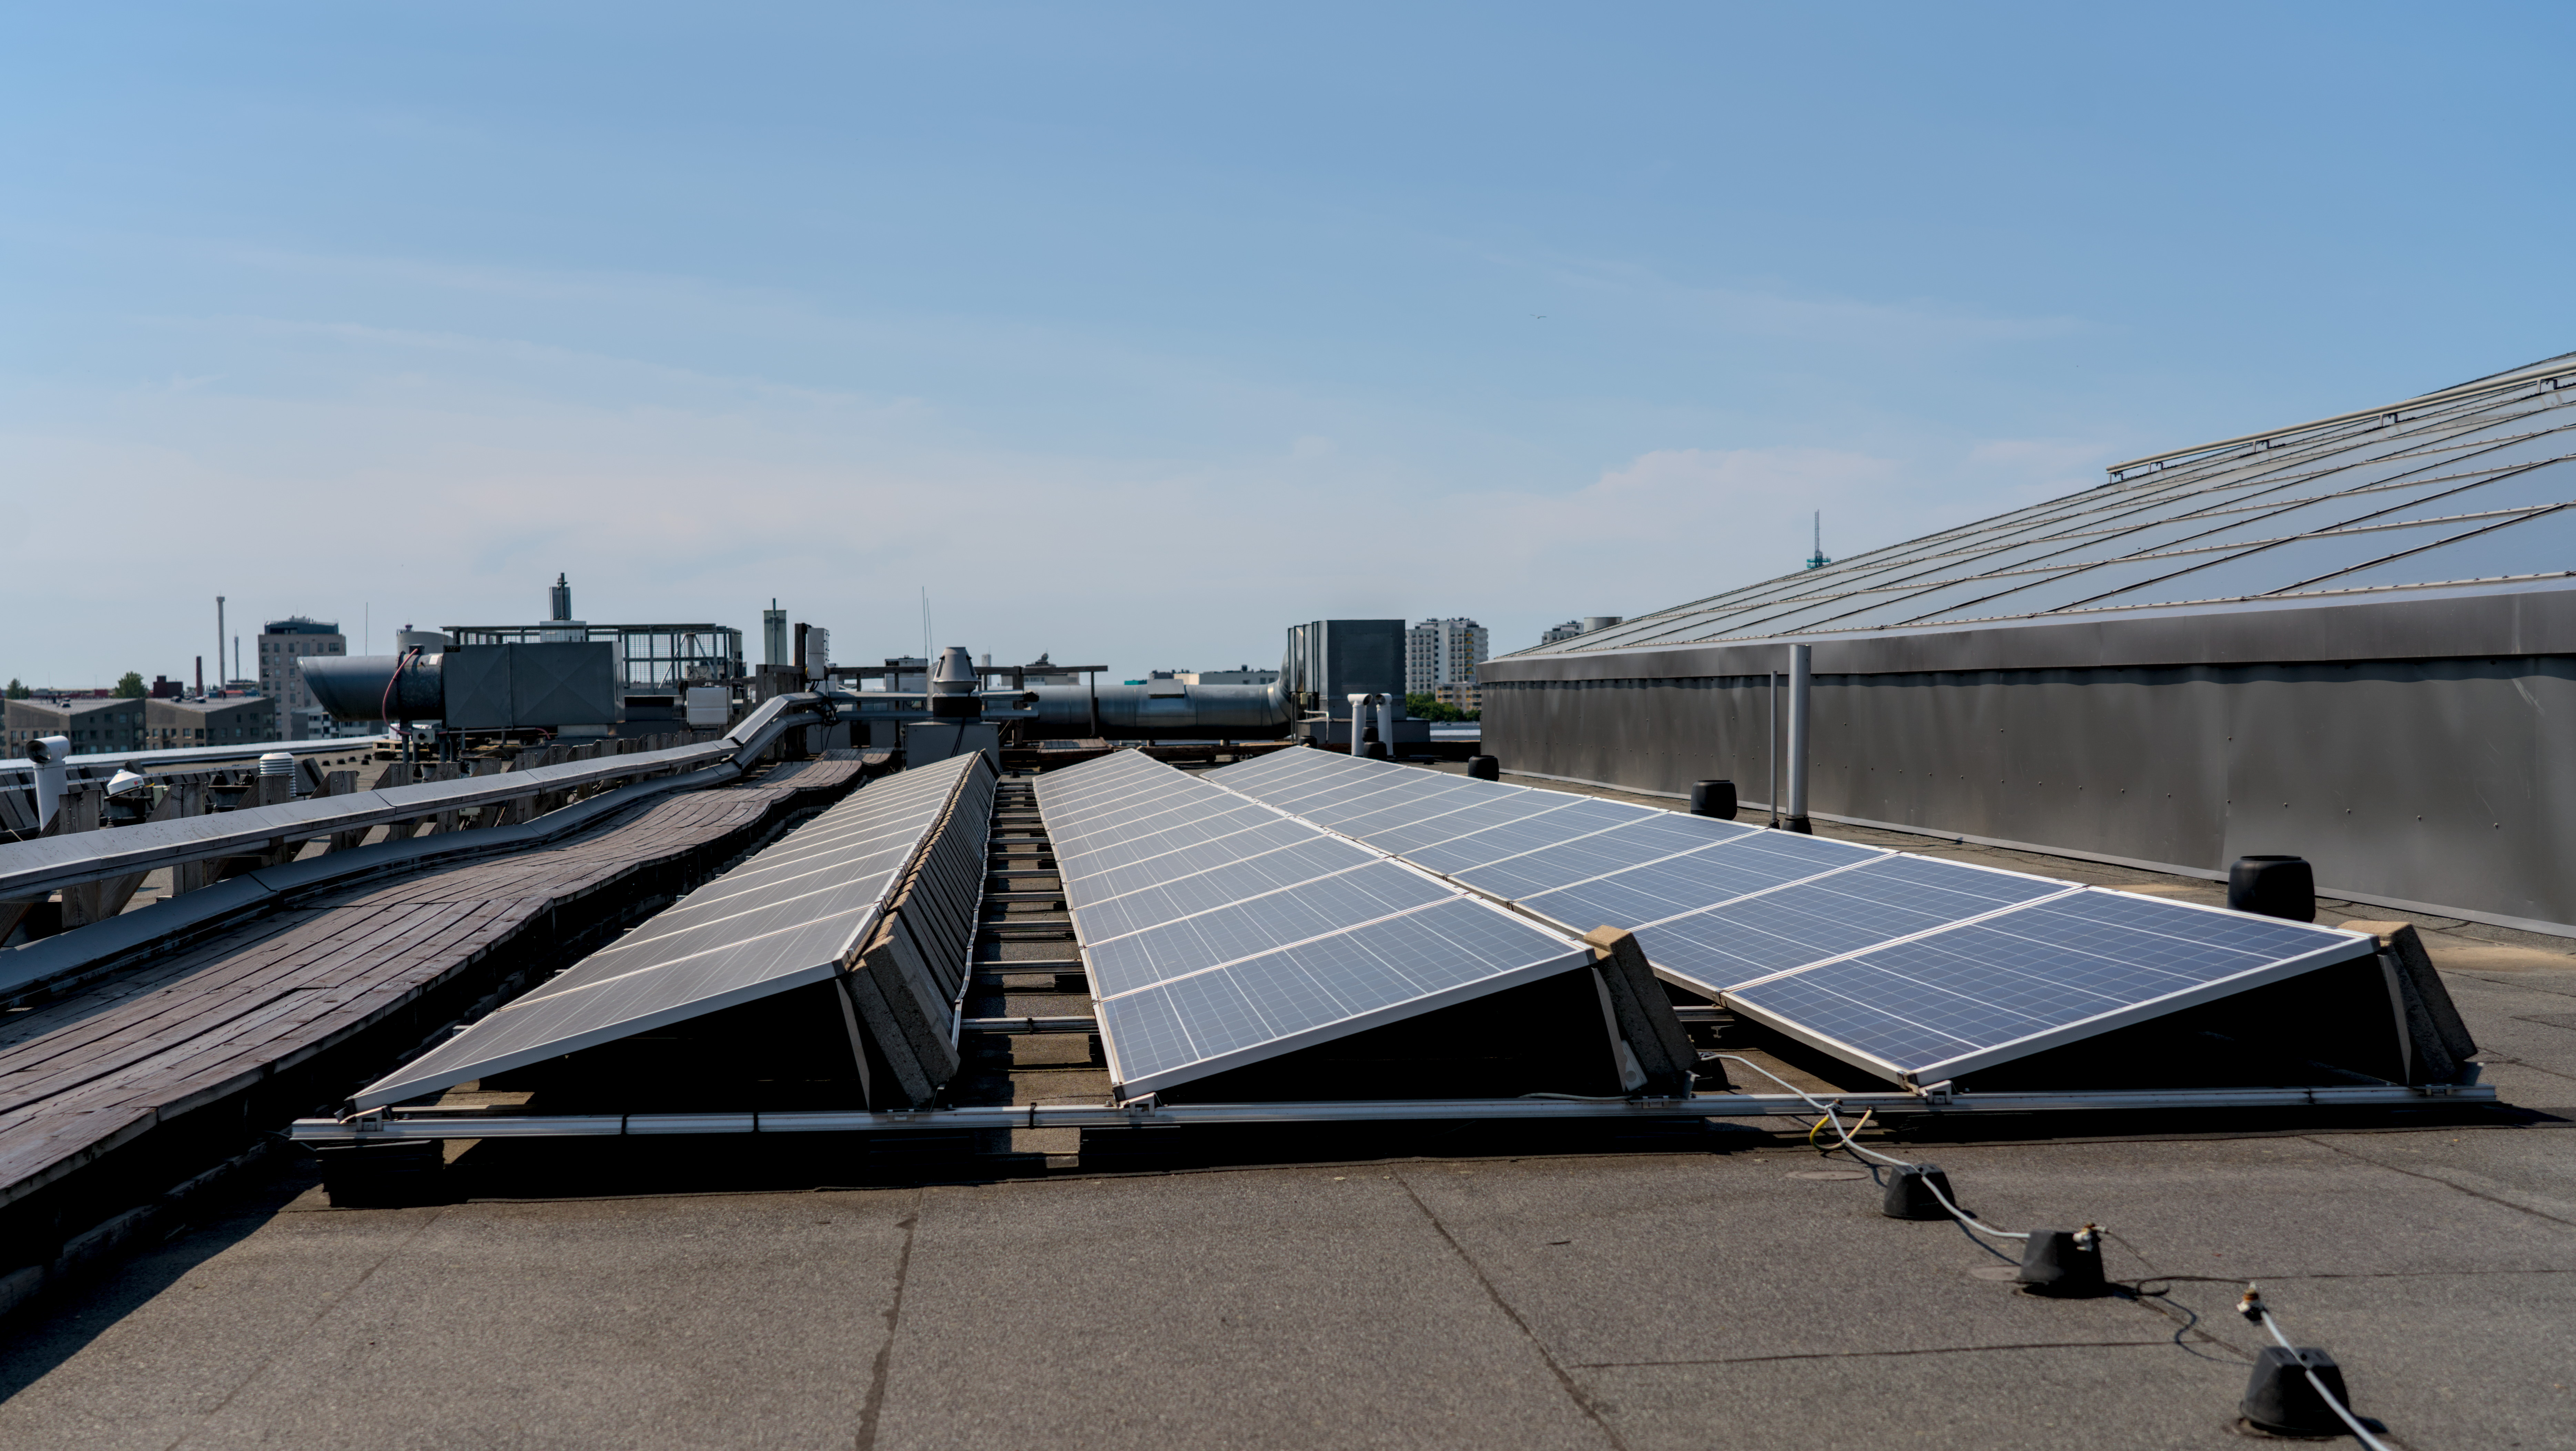
\includegraphics[width=0.8\linewidth]{pics/fmikumpula}
\figcaption{FMI Kumpula solar power installation string.}
\label{fig_fmikumpula_panels}
\end{figure}


\noindent The two datasets used in theis thesis were provided by FMI. They contain power generation measurements from installations in Kuopio and Helsinki, with the physical parameters listed in table \ref{table_fmi_helsinki_kuopio_parameters}. Due to the high elevation of the installations, shading is unlikely to be a major factor in either of the datasets. The same data was previously used in Herman Böök's \textit{Photovoltaic output modeling}\cite{hbook1} and thus installation parameters and datasets have previously been verified.

Data in the two datasets follows a similar structure as shown in table \ref{table_fmi_kumpula_csv}. This snapshot from the Helsinki dataset shows that the temporal resolution is one measurement per minute and that there are multiple power values for each minute. The fields \textit{String 1} and \textit{String 2} represent power from two identical sets or strings of solar PV panels installed at the same location and their sum should be near equal to inverter input. One of these strings is shown in figure \ref{fig_fmikumpula_panels}. Datasets from other sources may differ from the FMI datasets in several ways. Power measurements may be taken at different intervals, once per 1, 5, 15, or 60 minutes and they are unlikely to contain more than one power value. Due to these reasons, the algorithms in this thesis are designed to operate on datasets with one measurement per minute and they use only the inverter output value as that is the most likely power value included in solar PV datasets.


%Other datasets may differ from FMI datasets. The most likely differences are temporal resolution and the amount of included power measurement points. As the inverter output is the most important value for end users, this will be the only power value used by the algorithms. %The temporal resolution of one measurement per minute in FMI datasets is likely to be higher than that of most PV datasets, but  

% As these installations are used for research purposes, the temporal resolution and amount of power measurements are likely to be different from other solar PV datasets. Due to this, the algorithms in this thesis use the inverter output power value as it is the most likely power value to be included in datasets. The forementioned 


% As the inverter output describes the amount of power available to the user of a PV system, this will be used by the algorithms in the thesis. 


%ir data quality is likely to be higher than that of most regular solar PV installations. The multiple power measurements, installation metadata quality and 



%Having multiple power values has uses for data verification and analysis but the most relevant power value for the users of PV systems is the inverter output value and thus it is the value most likely to be included in datasets. 


%nother possible difference between FMI datasets and other datasets is the temporal resolution


%as the users of PV systems are interested in available power and thus inverter output values are the 


% only the inverter output value is likely to be included in solar PV datasets and thus it is the power value used in this thesis. Another possible difference between FMI datasets and other datasets is the temporal resolution as one measurement per minute 


% may be recorded anywhere from once per second to once per hour. Temporal resolution differences 
%The resolution of measurement per minute in FMI datasets should be accurate enough to allow for precise geolocation and panel installation estimation.




%have uses for analysis and data verification but are unlikely to be included in other datasets and thus algorithms in this thesis utilize only timestamps and inverter output values. Another likely difference between the datasets in this thesis and most real world datasets is the temporal resolution as power generation measurements may be recorded anywhere from once per second to once per hour. The resolution of measurement per minute in FMI datasets should be accurate enough to allow for precise geolocation and panel installation estimation.


\begin{table}[h]

\centering

\begin{tabular}{r|cccc} \hline\hline

Timestamp[UTC] & Inverter out & Inverter in & String 1 & String 2\\ \hline
$2015-08-26$ $03:34$ & $NaN$ & $NaN$ & $0.5$ & $NaN$\\
$2015-08-26$ $03:36$ & $11.1$ & $7.5$ & $2.6$ & $4.9$\\
$2015-08-26$ $03:37$ & $25.4$ & $26.1$ & $9.8$ & $16.3$\\
$2015-08-26$ $03:38$ & $30.7$& $NaN$ & $NaN$ & $0.4$\\
$2015-08-26$ $03:39$ & $46.4$& $44.8$ & $20$ & $24.8$\\
$2015-08-26$ $03:40$ & $3.3$ & $NaN$ & $NaN$ & $0.4$\\
$2015-08-26$ $03:41$ & $29.3$ &  $18$ & $9.1$ & $8.9$\\
$2015-08-26$ $03:42$ & $33.1$& $27.4$ & $10.6$ & $16.9$\\

\vdots & \vdots & \vdots & \vdots & \vdots\\
$2015-08-26$ $12:42$ & $12374.8$ & $14619.1$ & $7152$ & $7467.1$\\
$2015-08-26$ $12:43$ & $15442.2$ & $15482.1 $& $7708.9$ & $7773.2$\\
$2015-08-26$ $12:44$ & $14085.8$ & $12898.7$ & $6387$ & $6511.8$ \\
\vdots & \vdots & \vdots & \vdots & \vdots\\

\hline\hline
\end{tabular}

\tabcaption{A section from FMI's Kumpula solar site PV production data, only the timestamp and inverter output values are used by the algorithms in this thesis. All power measurements are in watts.}
\label{table_fmi_kumpula_csv}
\end{table}

%The same table shows that measurements for certain minutes are missing and that some values are recorded as NaN, Not-a-Number. Without proper preprocessing, mathematical operations such as sum, division and addition would be poorly defined and thus the dataset would be unusable. The required preprocessing is done by the removal of rows with NaN values and linear interpolation for filling out the resulting gaps. Filling gaps in the data is not necessary, but certain algorithms can be written more efficiently when no gaps are present.




%The table \ref{table_fmi_kumpula_csv} shows the general structure of solar PV energy output datasets with timestamps and power output values. The differences between FMI datasets and datasets from other sources are likely to be the timestamp formats, temporal resolution, power measurement units and the amount of different power measurement sources. Fields \textit{Inverter in}, \textit{String 1} and \textit{String 2} have uses for analysis and data verification but they or similar values to them are unlikely to be included in other datasets and thus this thesis utilize only timestamps and inverter output values.






%The algorithms in this thesis will work on any dataset with timestamps and power values, but the temporal resolution is likely to influence the accuracy of algorithms and interpolation has to be done in order to match the time resolution of measurements and the algorithms. The table also shows that the dataset is missing some values. In the case of the first and last daily minutes, this could be the result of the inverter or other instruments turning off when electricity generation is close to zero, but there could be other reasons as well. Due to the possibility of missing measurements and presence of NaN-values, the data has to be preprocessed. 


% similar data structures could be assumed to be the default in solar power generation datasets. The biggest difference between datasets could be assumed to be the temporal resolution, for example measurements for the power values could be taken every 15 minutes instead of every minute.



%Another point of interest are the multiple different power values included in the datafile. Columns String 1 and String 2 correspond to the output power from two identical sets of solar panels installed in the same installation site. Having two indentical installations at the same location has some value for data verification as both panel strings should provide almost identical outputs, but this is not the main focus of the thesis and thus these values are ignored. There are also two inverter values. The inverter input value is one step closer to the power generation of solar PV systems and thus algorithms that utilize this input value could be more accurate. However as the inverter output represents the amount of usable power generated by the PV system, the output is the most likely power value to be included in datasets and thus it will be used in this thesis.


%The table columns string 1 and string 2 correspond to the power outputs of two sets of panels. The output of these panels is used as the input of the inverter and thus the sum of string 1 and string 2 should closely match the inverter input value. The inverter is an electric device which converts the voltage of the solar panels so that the power generated by the solar panels can be fed into the electrical system of a home or some other facility.%As this output to an electric system is the best description of the power available to the user, an assumption can be made that the power value in other datasets refers to the inverter output unless otherwise indicated.



\begin{table}[H]
\centering
\begin{tabular}{r|cc} \hline\hline

 & Helsinki & Kuopio\\ \hline
 Latitude & $60.204^\circ$ & $62.892^\circ$ \\
 Longitude & $24.961^\circ$  &  $27.634^\circ$\\
 Nominal capacity &21 kW & 20.28 kW \\
 Panel tilt & $15^\circ$ & $15^\circ$ \\
 Panel angle & $135^\circ$ & $217^\circ$ \\
 Elevation & 17m & 10m\\
\hline\hline
\end{tabular}
\tabcaption{Parameters for the FMI's Kumpula(Helsinki) and Kuopio PV installations as listed in Böök 2020 \cite{hbook1}.}
\label{table_fmi_helsinki_kuopio_parameters}
\end{table}





\section{Visualizing the data}
The figure \ref{fig_oneyear_pointcloud} contains a 3D point cloud generated by plotting one year of data from FMI Helsinki dataset and it shows that there are patterns in the data. The clearest pattern is formed by the first and last non-zero power minutes and this pattern can be used for geolocation estimation. Similarly if one day slices from the dataset are taken as shown in \ref{fig_cloudfree_vs_cloudy}, the power generation plot shape can be later used for mathematical model fitting. However the difference between clear and cloudy or otherwise noisy days is significant and automating the process of cloud free day selection would be beneficial.



%free days is significant as seen in figure \ref{fig_cloudfree_vs_cloudy} and as cloudy or otherwise noisy days appear to be common in the data, automating the process of cloud free day selection is necessary.


%This shows that the timings of first and last non-zero power minutes appear to form a distinct pattern which is a result of changes in day length and this very same pattern can be used for geolocation estimation. If individual days from the dataset are plotted,



% Similarly the plot contains a noisy dome like-shape that can be used for analysis. In figure \ref{fig_cloudfree_vs_cloudy} we can see the the difference between different days in the dataset. This noise 



 %figure \ref{fig_cloudfree_vs_cloudy} 

\begin{figure}[h]
\centering
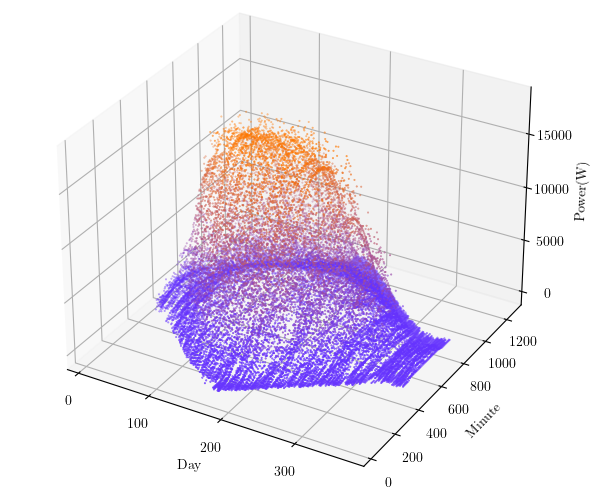
\includegraphics[width=0.8\linewidth]{pics/oneyear2}
\figcaption{One year of data from FMI Kumpula installation as a 3D point cloud.}
\label{fig_oneyear_pointcloud}
\end{figure}

\begin{figure}[h!]
\centering
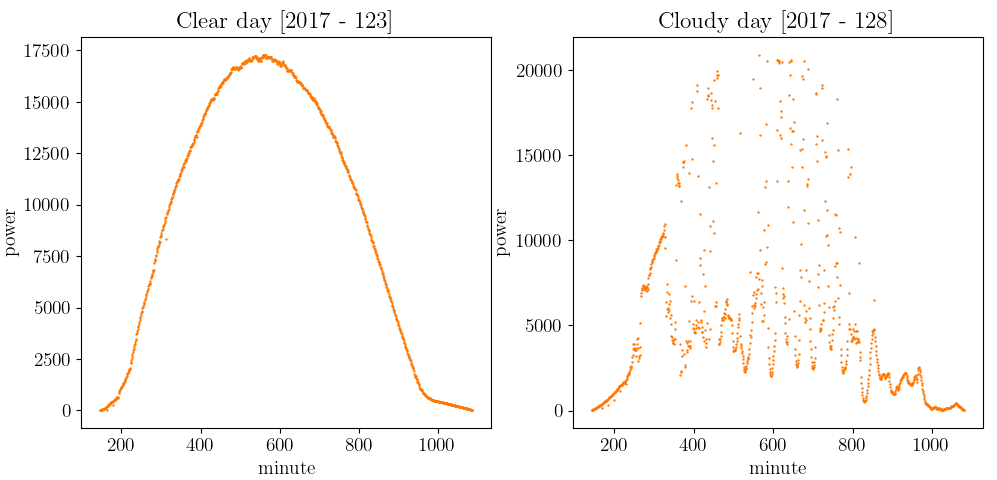
\includegraphics[width=1\linewidth]{pics/cloudfree_vs_cloudy}
\figcaption{Two days from FMI Kumpula dataset with different charasteristics.}
\label{fig_cloudfree_vs_cloudy}
\end{figure}

The cloud free day 2017-123 has some notable charasteristics in addition to the geolocation derived first and last minutes. The shape resembles a skewed normal distribution and the knee section near 950 minutes may signify a transition from direct solar irradiance to atmosphere scattered irradiance. Similarly intuition would suggest that the peak power minute is near the time when the angle between sun and the solar panel normal is at it's minimum. Measurable traits such as these could be used for parameter estimation, but the relationships between figure traits and system parameters can be complicated.



\newpage
\section{Data pre-processing}
The data pre-processing required by the algorithms in this thesis can be split into two gategories, classification and repairing. Classifying preprocessing is used to determine if a certain section of data is useful of analysis or not, the primary example here is the cloud free day detection algorithm which is discussed more throroughly in the next chapters. The second type of preprocessing, reparing preprocessing refers to the use of algorithms which fill in gaps or otherwise attempt to repair data which is unusable as is, but which could be used after repairing.


% Similarly algorithms can classify days as good and bad based on their measurement counts, legths or data gaps. 

The data preprocessing algorithms used in this thesis load the data from csv files and examine whether individual days in the dataset meet set qualifications. These are the minimum and maximum measurement count, whether first and last measurements are taken too close to minute 0 or 1440 and the the percentage of measurements included between the first and last measurement. Figure \ref{fig_accepted_days} shows which days met the set quality requirements.



\begin{figure}[h]
	
     \centering
     \begin{subfigure}[b]{0.48\textwidth}
         \centering
         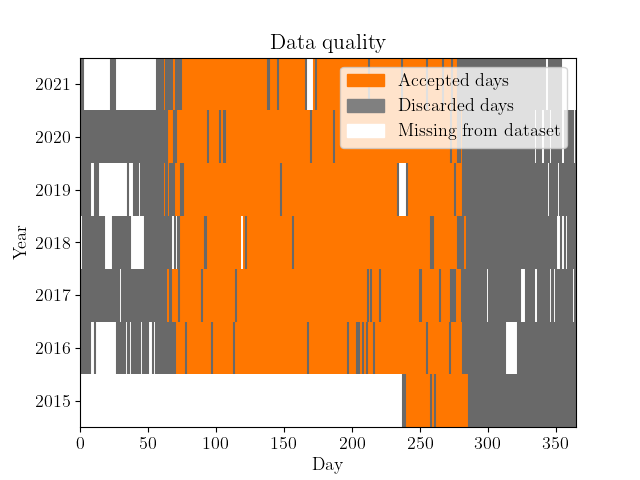
\includegraphics[width=\textwidth]{pics/helsinki_accepted_days}
         \caption{Days in Helsinki dataset which met data quality thresholds.}
         \label{fig_helsinki_accepted}
     \end{subfigure}
     \hfill
     \begin{subfigure}[b]{0.48\textwidth}
         \centering
         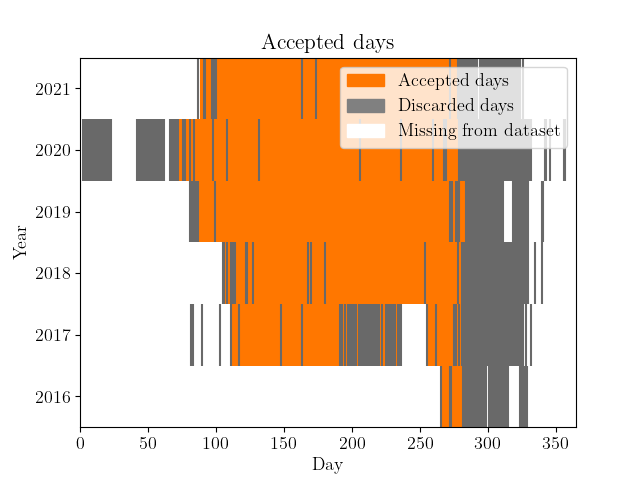
\includegraphics[width=\textwidth]{pics/kuopio_accepted_days}
         \caption{Days in Kuopio dataset which met data quality thresholds.}
         
         \label{fig_kuopio_accepted}
     \end{subfigure}
     \hfill
     \caption{Visualizations of data quality. Measurement count between 400 and 1200, first minute is 5th or later, last minute is 1435 or earlier. More than 95\% of measurements between first and last minute must be included.}
     \label{fig_accepted_days}
     
\end{figure}


After acceptable days are chosen with the classification algorithm, the next step is data repairing. Missing measurements and Nan values can be linearly interpolated, meaning that if a power measurement or a set of measurements is missing between two datapoints, the missing datapoints are estimated to describe a linear transition breaching the gap between the known datapoints. When noise level is low, linearly approximating the missing values is unlikely to result in signficant errors. After this is done, the resulting data is ready for analysis.

% One issue with the described preprocessing methods is that they do not take into account strong longitude induced shifts which may be present when installation longitudes strongly deviate from 0$^\circ$. For example, at zero degrees longitude a 12 hour day would begin at around 360 minutes and end at 1080 minutes. If the longitude is shifted by $\pm 90^\circ$, the 





%These days are then repaired by creating new days with 1440 power measurements where power at minute $i$ is the power measurement from the dataset if such measurement exists. If not, the power is defined to be 0 when outside the range of first and last non-zero measurement of the day and $Nan$ if whitin. The resulting day after these steps is defined at every minute of the day but it may still include gaps filled by $Nan$-values. These gaps 





%can be used for filling gapps in otherwise good data or for other data processing where the data is nearly usable but some modifications are needed.


%cloud free days and the topic will be better explained in the next section


%The not-a-number or $NaN$ values visible in the table \ref{table_fmi_kumpula_csv} could cause issues with some data processing algorithms. In the python programming language, many mathematical functions will always return $NaN$ if even a single $NaN$ value is present in the input. Another issue with datasets is that they include gaps, meaning that rows corresponding to some minutes are not present in the dataset. If these gaps are significant enough, their existance could causes errors and biases in processing algorithms.

%If significant amounts of measurements are missing between the first and the last measurement of the day, this could result in biases and errors with processing algorithms.


%This means that unless $NaN$ values are filtered out, a significant amount of mathematical functions will not return expected real values. Another issue with datasets is that they could include gaps, meaning that rows corresponding to some minutes are not present in the dataset. If significant amounts of measurements are missing between the first and the last measurement of the day, this could result in biases and errors with processing algorithms. %For example if a significant amount of measurements is missing, estimating the area under the plot in graphs such as \ref{fig_clearday} by simply taking the sum of the power outputs would result in underestimating the actual power output. And the more values are missing, the stronger the error would be. 

%One solution for this problem would be to design every algorithm to accept two inputs, the measured power and the measuring time but this would come at a cost to algorithm complexity. The easier option and the method used for processing the FMI datasets is the removal of all rows with $NaN$ power values and the use of linear interpolation in order to approximate the missing rows. In this case linear interpolation is applied on the minute dimension, meaning that if a gap in power measurements is detected on the minute axis, the missing minutes are filled so that the gap is filled with a linear transition breaching the gap.








\section{Clear day detection algorithm}
\label{clearskyalgo_chapter}
While the previous preprocessing steps have filtered and repaired days according to measurement counts and data gaps, these algorithms did not take the quality of measurements into account. If the interference in measurements caused by clouds or other sources is significant, the value of a day for model fitting is reduced. An example of strong interference can be seen in figure \ref{fig_cloudfree_vs_cloudy}. Detecting the presence of such interference with an algorithm would help with automating the process of model fitting as that would eliminate the need to manually select good days from datasets. The following is an explanation of how the cloud free day detection was accomplished in this thesis.




% It should be apparent that the cloudy day is not as useful for model fitting as the clear day and thus an algorithm for automating the process of detecting clear days is needed. The following steps describe the process of cloud free day detection.



%These cloud free days are visually distinct from cloudy days \ref{fig_cloudfree_vs_cloudy} and their algorithmic classification as cloud free helps in automating the parameter estimation process further. The following list is a step by step description of a such algorithm.


%\noindent \textbf{Algorithm step by step:}

\begin{enumerate}
  \item Separate the dataset into individual days.
  
  \item Create a copy of the day and apply a low pass filter to the power measurements of the copy.
  
  \item Measure the smoothness of a day by measuring how significant the changes induced by the low pass filter are.
  
  \item Discard days which fail to meet a set smoothness threshold. Remaining days are likely to be cloud free.
  
  
  
   %If the average difference from step 5 is on average higher than a given treshold value, reject the day.
\end{enumerate}



\noindent The mathematically non-trivial parts here are the threshold selection, difference measurement and low pass filtering. Low pass filtering is a term borrowed from the field of signal processing and it refers to any algorithm which removes frequencies higher than a given limit from a signal, allowing lower frequencies to pass. 



Here the filtering is done with the help of discrete Fourier transformations and inverse discrete Fourier transformations. Discrete Fourier transformation transforms a given list of numbers to a set of sine and cosine equations which approximate the given input, this trigonometric approximation can then be reversed in order to return the continuous trigonometric approximation back into the original discrete values. As the output of a discrete fourier transformation is ordered, by modifying the output of the transformation, frequencies can be selectively removed or amplified. By zeroing out all but the n longest frequencies, we can generate a smooth continuous approximation of the given input. By then reversing the modified continuous approximation back into a list of discrete values using inverse discrete Fourier transformation, we have a way of filtering high frequencies from a list of numbers. An example of what this looks in practice is shown in figure \ref{fig_cloudfree_algo} where the 6 longest frequencies were used for approximating the discrete datapoints. 

Note that while this process is somewhat complicated, Fourier transformations are not the only tool for creating low pass filters. Similar results can also be achieved by locally averaging each power value to be the average of nearest k values. Discrete Fourier transformation based methods do however have an advantage in their universality. If the 6 or 7 or n longest frequencies can be determined to be a good low pass filter, then these same frequencies should result in similar outputs no matter the temporal resolution of the power measurement data. Where as a method based on local averages would require more tuning.

The second component is not as complicated. Measuring the delta between a filtered and unfiltered set of measurements can be done by computing the discrete curve length or as was done here, measuring the absolute average deviation between filtered and unfiltered power measurement. This is shown with the following equations 2.1-2.4.


\begin{align}
Power &= [p_0, p_1, p_2, \dots , p_n] \\
Power_{filtered} &= [f_0, f_1, f_2, \dots , f_n] \\
Power_{delta} &= [|p_0 - f_0|, |p_1-f_1|, |p_2-f_2|, \dots , |p_n-f_n|] \\
delta_{avg} &= avg(Power_{delta}) \\
delta_{norm} &= delta_{avg}/ max(Power)
\end{align}


The last component is threshold selection. By choosing to reject every day for which the $delta_{norm}$ value is higher than 0.05, we can eliminate days where measurements deviate on average more than 5\% from the low pass filtered measured power values. With the Helsinki and Kuopio datasets threshold values as low as 0.5\% still provided some outputs. This is unlikely to hold for other datasets as differences in temporal resolution and installation specific shading patterns are likely to change the noise patterns in data. 


%The thresholds between datasets are not directly comparable. Installation specific shading patterns may increase the base level of noise present in datasets and thus higher thresholds 



%While the The algorithm has some weak points. 



%As the method is based on calculating the delta from a smooth approximation, percentual delta values are unlikely to approach zero unless the modeled data itself is faulty. Depending on the data quality, higher threshold values may need to be used. For example, if the panels are shaded by a tree or some other obstruction during a short period each day, then base level of noise in the measurements would be higher than it is for the FMI datasets. 


%This could be circumvented by 


%As the algorithm is designed for finding the very smoothest of days, the algorithm generates large amounts of false negatives. When this is combined with the interference from sources other than clouds, 


%, the high number of false negatives 


%And as it is designed to seek the very smoothest of days, resulting in a large amount of false negatives. In addition, other forms of interefence such as snow on panels, reflective surfaces near solar panels and clouds which do not block direct sunlight may distract the algorithm. From a human perspective the results of the algorithm may thus be unintuitive as a snowy day may be classified as cloudy even though the interference source was snow on the panels and not the cloud cover. But from the perspective of the processing algorithms, the source of noise in the data is irrelevant.

%Despite these differences


%The terms used in signal processing have mathematical counterparts with some distinctions, for example we can use mathematical structures such as lists, matrices or graphs as signals. And the mathematical near equivalent of high and low frequencies could be defined with the help of delta values between neighboring numerical values in these structures. If the delta values between any two near by values is significant, then this section of the mathematical structure contains high frequency change. Similarly if delta values between any two distant values are high, this is indicative of low frequency change between these two points.






%\noindent There are two mathematically non-trivial components in the algorithm. The first is low pass filtering, a process which treats cloudy and cloud free days differently. This is a concept borrowed from the field of signal processing and the differential treatment can be used to aid in classification. The second non-trivial part is measuring the change between filtered and unfiltered measurements. If the change is minimal, the day can be classified as cloud free.

%The term low pass filtering can be used for any process which takes an input and eliminates frequencies which are higher than a chosen cut off frequency, allowing lower frequencies to pass. With the power measurements, a simple low pass filter could be a running average filter which calculates a new power value as the average of the last $n$ values. The low pass filtering used in this thesis and shown in \ref{fig_cloudfree_algo} was accomplished with discrete Fourier transformations. Discrete Fourier transformations change a list of numbers into a set of sine and cosine waves of different amplitudes, the sum of which forms a continuous representation of the discrete values. This continuous representation can be sampled in order to return the data back into discrete values and by selectively choosing only the waves with longest wavelengths, discrete Fourier transformation can be used for low pass filtering. Good results were achieved by using the 5 to 7 of the longest frequencies generated by the fast Fourier transformation algorithm. 

% n-th degree polynomial approximation of the measurements or new and filtered measurement values could be defined as the average of nearest 20 power measurements.


% The second non-trivial component is measuring the delta between filtered and unfiltered days. This is accomplished by calculating the lenghts of point to point curves in Euclidean space represented by the measurements and filtered measurements by using the equation $\Sigma_{i=1}^{n}  \sqrt[2]{1+ (powers[i]-powers[i-1])^2}$. If the curve lenghts differ by more than x percent, the day can be classified as cloudy.

%The second non-trivial component is measuring the delta between filtered and unfiltered days. This is accomplished by first computing the per minute delta $\delta[i] = |p[i] - p_{lp}[i]|$ where $p[i]$ is the measured power value at index $i$ and $p_{lp}[i]$ is the corresponding power measurement after low pass filter was applied. These delta values can then be used for calculating the average delta per measurement $\delta_{avg} = (\delta[1]+\delta[2] + \dots+ \delta[n])/n$. This normalization is important as without normalization days with lower temporal resolution or shorter day lengths would have lower delta values. The delta value $\delta_{avg}$ can be normalized further as $\delta_n=\delta_{avg}/p_{max}$. This final normalization step results in a delta which represents per measurement deviation as a fraction of max and this final value is comparable between installations of different sizes.

%Final part of cloud free day detection is choosing a threshold value. By manually testing different threshold values, the lowest values which still returns days with the Helsinki and Kuopio datasets are 0.3 and 0.5 respectively. This difference is small but it shows that there is a measurable difference between the datasets and that threshold value should be chosen based on the datasets used. Another issue with the algorithm rises from temporal resolution, if temporal resolution is 1 measurement per 15 minutes and if the reported value is an average of last measurement period, a low pass filter has already been applied. This would not make the algorithm unsuitable for its purpose, but threshold values would have to be adjusted. One method for generalizing the algorithm and avoiding the forementioned issues would be sorting the days based on their smoothness values and then choosing the $n$ smoothest days to operate on. Such modifications may be necessary or beneficial when operating with large amounts of different datasets, but as of now they have not been implemented.


%Most of the program code required for cloud free day detection is included in appendix \ref{cloudfree_code} and the complete source is available on github \cite{github_source}.

%s based on their apparent smoothness values and then operating with the 

%The second non-trivial component is measuring the delta between filtered and unfiltered days. This is accomplished by calculating the lenghts of point to point curves in euclidean space represented by the measurements and filtered measurements by using the equation $\Sigma_{i=1}^{n}  \sqrt[2]{1+ (powers[i]-powers[i-1])^2}$. If the curve lenghts differ by more than x percent


%length of a day by calculating euclidean distance over a day of measurements with the sum function: $\Sigma_{i=1}^{n}  \sqrt[2]{1+ (powers[i]-powers[i-1])^2}$



%Here the algorithm first computes the per measurement error $\delta_i$ for each measurement $p_i$ in the list of powers so that $\delta_i = |p_i - {p_i}_{lp}|$ . This results in a new list of error values is then used in orde to compute the average deviation from 



%Then the average deviation is calculated $\delta_{avg} = (\delta_1+\delta_2 + \dots+ \delta_n)/n$. Finally the delta can be normalized to 



%Here the chosen method is based on computing the length of the discrete curve in minute-power space and the equation used is the sum of point to point distances in Euclidean space. The 



%Alternative approaches such as measuring the total travel on power-axis and calculating error area between filtered and unfiltered curves could also be used. 










%The algorithm splits data into individual days of measurements and the days are evaluated separately. This means that 

%Another important form of data pre-processing is the selection of days which are suitable for model fitting. These so called cloud free or clear days can be distinguished by their smooth power measurement curves as seen in \ref{fig_cloudfree_vs_cloudy}, but the strength of cloud induced noise can be stronger or weaker as well. By making the assumption that clouds induce randomness into the power measurements, we can attempt to measure this randomness and use it as a metric for deciding whether a day is suitable for model fitting or not.

%\noindent To borrow terminology and tools from the field of signal processing, a clear difference between cloudy and cloud free days is the presense of high-frequency noise. Noise means that the alteration to the signal is unwanted and high-frequency signifies that the alteration results in a signal where measurements differ from neighboring measurements. In the case of solar PV power measurements, power $p_t$ for minute $t$ is more likely to differ from the average of the nearest 10 or 100 measurements if the day is cloudy than when the day is cloud free. This difference is visible in \ref{fig_cloudfree_algo} where a cloud free and cloudy day have both been locally averaged.

%Locally averaging or low pass filtering the values can be done in multiple ways. For example, the filtered values could be defined as the average of the nearest 50 values or a polynomial of sufficient degree could be fitted to the measurements data. Regardless of the method used, the important aspect is that the averaging function has to eliminate the apparent randomness from the signal while cloud free days should be hard to distinguish from their unfiltered counterparts. 

%Here the chosen low pass filtering method uses discrete Fourier transform. Fourier transformations are a method of representing number series and functions as sine and cosine waves. In short, the sum of a sine and a cosine wave of frequency $f$ can be used to construct a new sine wave of frequency $f$ with chosen phase. Fourier series combine this property and multiple frequencies in order to construct a frequency representation of the approximated data. As Fourier transformations start from the computation of the longest frequencies, the first $n$ outputs can be used to approximate the general shape of the data.

%This method of filtering may seem complicated as the same results could be achieved by defining new power values as $p_{t_{new}} = avg(p_{t-n}, ...,p_{t-1},  p_t,p_{t+1}, ..., p_{t+n})$ but this would require the turning of the window size parameter $n$ which is dependent on temporal resolution. The benefit of the Fourier series based method is that it is independent from temporal resolution and unlike Taylors polynomial or other localized approximation methods, discrete Fourier series approach does not favor a certain data interval.


\begin{figure}[h]
\centering
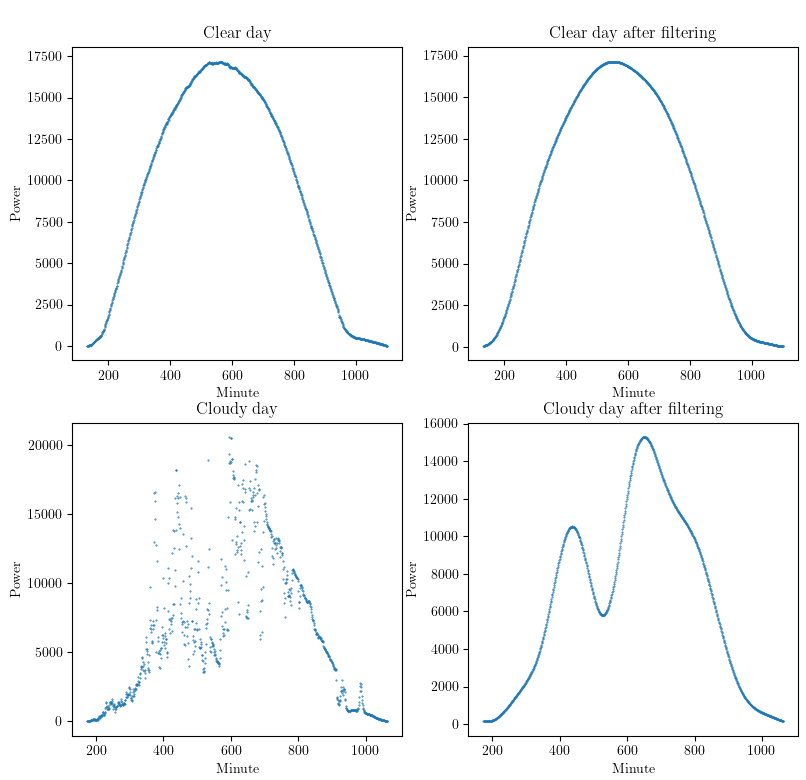
\includegraphics[width=0.8\linewidth]{pics/cloudfree_algo}
\figcaption{Cloud free day finder low pass filtering phase.}
\label{fig_cloudfree_algo}
\end{figure}



\newpage






%\noindent \textbf{Note:} that the algorithm listed above is highly dependent on measurement intervals and further tuning could be needed when operating with datasets that have different temporal resolutions. And as is, the algorithm selects days based on their proportionally low high frequency component, thus in theory this algorithm should classify zero power output days as cloud free days. Despite this fault the algorithm seems to work well for the FMI datasets.% as long as the input are selected to contain days close or between the spring and fall equinoxes. 



%The implementation of the clear sky algorithm seems to work well as indicated by \ref{fig-multidaypoavsmeasurements} but there are a few weak points in the algorithm as well. For example if a constant power day is given as the input for the algorithm, the algorithm will classify it as clear sky day even if a constant power day is more likely to be the result of faulty measuring instruments or errors in data preprocessing than a real cloud free day. In addition, the algorithm is unlikely to work well if sections are either removed from the measurements or if there is significant shading affecting the power output of the installation.

%\subsection{Difference between solar days and UTC days}
%For solar power analysis the concept of solar days is fairly useful. Solar days and sun based time measurement systems tend to rely on the angle of the sun and three 


%The timestamps used in solar PV measurements can be assumed to be in UTC +0 time. While this means that timezones or daylight saving time do not have to be accounted for, some operations may become more complicated as well since UTC days and solar days at do not always align. Note that here local solar day is defined as the 

%For example, if a one day slice is taken from a $0^\circ$ longitude installation power generation data, it is rather likely that the solar power generation would occur during an interval which centers around noon or 720 minutes. If the same slice is taken at $90^\circ$ longitude, this generation would be shifted by approximately 360 minutes. This is perfectly normal and expected behavior, but as a result, determining the first and last non-zero minutes of the day can be seen to nontrivial as per figure \ref{fig_poa0vs90}. In the $0^\circ$ plot, the first and last non-zero minutes are approximately 330 and 1100, but should the first and last minutes of the $90^\circ$ plot be defined as 0 and 750, 0 and 1420, -19 and 750 or something else entirely?


%\begin{figure}[h!]
%\centering
%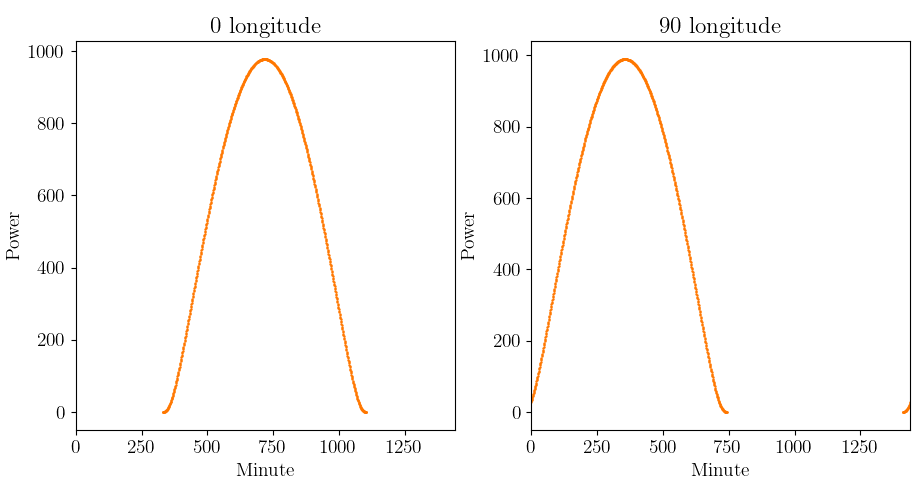
\includegraphics[width=0.9\linewidth]{pics/poa0vs90}
%\figcaption{Approximations of solar power generation at $0^\circ$ and $90^\circ$ longitude.}
%\label{fig_poa0vs90}
%\end{figure}


%\section{Third party datasets}
%Sunny portal etc here

%\section{Required assumptions}The algorithms presented in this thesis work on datasets which 


%Due to the diversity of possible solar PV installations, creating an universal model for parameter estimation is not fesiable. Installations could have been modified during operation, system failures could induce different types of changes in measurement data and 




%\section{Assumptions and possible issues}
%If metadata such as the geographic location or panel installation angles is missing from the datafiles, it is very likely that other critical pieces of information could be left out as well. Were additional modules were installed during operation? Could some panels be installed at different angles? What if the panels are installed in tracking mounts and thus the panel angles vary during each day? These questions are left unaswered and thus some assumptions have to be made. In this thesis we will assume that the panels are installed on fixed mounts, no changes were done during data gathering period and all panels are oriented similarly. We will also assume that there are no major obstacles casting shadows on the panels and that the panels are not self-shadowing, meaning that the panels are not casting shadows on one another.

%Another source of uncertainty is data collection itself. The device responsible for measuring power output values and logging the values has to have a clock for measuring time, but this clock could have be running too slow or fast, resulting in a drifting error in the timestamps. Similarly if the system clock is running at the right speed but it is off by a minute or two, this could cause a bias in the data which would be hard to detect. There is also the question of how measurement timing is done. If the time resolution of the logging device is 15 minutes, is the power value at 12:45 taken during the 45th minute or is the power value the average of the previous 15 minutes as is often done in meteorology? Or could the power value be the average of measurements taken during the interval 12:38 to 12:52? In meoteorology, the last period average would be the standard, but standards may not always be followed.

%is the standard, but standards are not always followed and thus 

%If enough time and effort was spent on algorithm design, in theory it could be possible to detect modifications to PV systems, the presence of variable panel angle systems and clock drifts. But these topics are outside the scope of this thesis and thus the assumption will be made that the 






















\chapter{Solar irradiance simulation tools}
Having a mathematical model which would simulate the output of a PV system would allow for the parameters of a PV installation to be solved with model fitting. In the best case scenario, we would have a physics based model which would take geographic location, panel installation angles, time of year and panel surface area or power rating as inputs and the output would be similar to the data from FMI Kumpula installation seen in table \ref{table_fmi_kumpula_csv}. Creating a such model is rather challenging as the model has to take into account atmospheric scattering, Sun angles, Sun-Earth distance variation and a multitude of other factors, the consideration of which are far beyond this mathematics thesis. Luckily the modeling of the energy output of solar PV installations has uses for the cost-benefit analysis of solar PV installations and thus pre-existing modeling algorithms are publicly available. 


% TODO REWRITE

This thesis uses a plane of array irradiance simulation function from the python library PVlib. The function takes geographic location, timestamp and panel angles as inputs. The outputs contain power values which describe the amount of direct and atmospherically scattered light that would hit a square meter sized imaginary solar panel with the input parameters. The sum of these sources is referred as plane of array (POA) irradiance and this value can be used to estimate the output of solar power installations. A section of simulated data is included in table \ref{table_poa_simulated_format}.

As the model simulates radiation values during clear sky conditions and not the power output of pv installations, the model should be seen as an approximation which is accurate to a certain degree. The differences between the model and recorded measurements could be due to reflectivity of the solar panels, weather conditions, temperature related changes in efficiency, atmospheric composition or a multitude of other factors which the model does not take into account.

\begin{table}[h]

\centering

\begin{tabular}{r|cccc} \hline\hline

Timestamp[UTC] & Minute & POA(W) \\ \hline
$2018-05-30$ $00:00$ &  $0$ & $0.0$\\
$2018-05-30$ $00:01$ &  $1$ & $0.0$\\
$2018-05-30$ $00:02$ &  $2$ & $0.0$\\
\vdots & \vdots & \vdots \\
$2018-05-30$ $ 07:34$ & $454$ & $800.691861$\\
$2018-05-30 $ $07:35$ & $455$ & $802.110516$\\
$2018-05-30 $ $07:36$ & $456$ & $803.517424$\\
\vdots & \vdots & \vdots \\
$2018-05-30$ $ 23:57$ & $1437$ & $0.0$\\
$2018-05-30 $ $23:58$ & $1438$ & $0.0$\\
$2018-05-30 $ $23:59$ & $1439$ & $0.0$\\

\hline\hline
\end{tabular}
\tabcaption{One day of simulated plane of array irradiance values. Note that the minute column is added to the table for convinience and it is reduntant as minutes can be read from the timestamps.}
\label{table_poa_simulated_format}
\end{table}

\section{PVlib POA python function} % , parameter space and computational requirements}
Taking a look at the code responsible for the plane of array irradiance simulations can give some insights into the behavior of the estimations and problem of parameter estimation. The  python function responsible for simulating plane of array irradiance values over a day is defined with the header \ref{poa_header}. In this header we can see that the function takes 7 inputs each of which is mandatory, meaning that when the functions is used as a tool for parameter estimation, some of the parameters have to be guessed or randomly assigned.

\begin{lstlisting}[caption={PVlib POA simulation function header.}, label={poa_header}]
def get_irradiance_with_multiplier(year, day, latitude, longitude, tilt, azimuth, multiplier):
\end{lstlisting}







%The following python code is a function which adds the ability to scale the power values of PVlib POA simulations. This ability is needed as by default PVlib simulates the amount of energy radiated towards an imaginary square meter sized solar panel with given coordinates, timestamp and installation angles and as such the power values have to be scaled in order to match the surface areas and efficiency of real installations. The code itself does not tell much of the mathematics used for the simulation, but it can be used to show the input parameters required by the POA simulation function. Each of the 6 parameters is mandatory, meaning that if latitude, longitude, day or any other parameter is left out when the function is called, this will raise an error upon code execution. This means that when the functions is used as a tool for parameter estimation, some of the parameters have to be guessed or randomly assigned. 

%This wrapper shows that six input variables are used for generating a day long POA simulation. The functions requires these parameters, meaning that python will raise an error if the function is called without the necessary 6 inputs. This means that when the function $get\_irradiance\_with\_multiplier()$ is used as a tool to solve the parameters of a system, up to 5 parameters may have to be guessed or assigned random values. The parameters and their ranges are as follows:
\subsection{Function input parameters} 
The following listing contains the parameters of the plane of array irradiance function and their domains.
%The POA simulation function accepts real --or integer as is the case with the day parameter-- valued parameters in the ranges listed below. 

\begin{itemize}
	\item Year $\in \mathbb{N}$
	\item Day [1, 365/366] $\in \mathbb{N}$
	\item Latitude [-90, 90] $\in \mathbb{R}$%, Finland fits within subrange [59, 70]
	\item Longitude [-180, 180]  $\in \mathbb{R}$%, Finland fits within subrange [19, 32] 
  	\item Tilt [0, 90] $\in \mathbb{R}$
  	\item Azimuth [0, 360[ $\in \mathbb{R}$
  	\item Multiplier ]0, $\infty$[ $\in \mathbb{R}$
\end{itemize}

%\noindent \textbf{Note:} While the function does accept the full latitude and longitude ranges as inputs, it may be beneficial to restrict the range of the coordinate parameters when the approximate location of the installation is known. For example, Finland fits within subrange [19, 32] on the longitude axis and thus it could make sense to restrict the longitude range when examining installations located within Finland.

\vspace{3mm}
\noindent The combination of these parameters and their ranges can be thought to form a subspace in seven-dimensional Euclidean space, or six dimensional if year and day are combined into a date variable. This so-called parameter space and its "volume" are both concepts that can be used for analyzing the difficulty of parameter estimation problems, behavior of parameter estimation functions and their efficiency. In general, the more parameters and thus dimensions there are, the larger the resulting parameter space is and the harder the problem becomes. And the more parameters an algorithm is attempting to solve at once, the slower the algorithm can be expected to be.

With solar PV installation parameter estimation, there are 5 unknown parameters as the year and day parameters are always known. If each of the remaining parameters is discretized to 20 evenly spaced values, solving all the 5 parameters at once by testing out every possible combination would require evaluating $20^5$ or 3.2 million unique combinations. However if the parameters could be solved one by one, isolted from the influence of other parameters, there would only be $20*5$ or 100 unique combinations, a reduction of 32000 to 1. This highlights how important it is to break larger problems into smaller problems whenever possible.

%In the worst case where none of the 6 parameters are known and each of the parameter space axes are discretized to $n$ unique evenly spaced values, then the amount of possible combinations is $n^6$. 

%The exponent of 6 may seem insignificant, but even with a crude space discretization where $n$ is chosen to be 20 would result in 64 million combinations. If testing out one parameter combination were to take a second of computing time, testing out each of the 64 million combinations would require more than 700 days of non-stop computing. Luckily the day parameter is always known and thus $n^6$ drops into $n^5$ but even then the size of the parameter space is enormous.

%Thus the goal of the parameter estimation functions should be to reduce the freedom of movement in the parameter space as efficiently as possible, eventually restricting the parameter space into an individual point which corresponds to the installation parameters of the system.


%This means that when unknown parameters of a multi parameter function are being solved, emphasis should be placed on solving the parameters one by one


%In best case scenario, one or more of these parameters can be locked to a specific value. This decreases the volume of the parameter space and the goal 


%the amount of different parameter combinations that may have to be tested while the installation parameters are being solved. 



%The amount of dimensions is relevant as if $n$ discrete values are chosen for each parameter, the total amount of different parameter combinations would be $n^6$. Luckily the day parameter is always known and thus there are only 5 free dimensions, but this still results in a fairly large parameter space. Even a crude discretization with 20 values per dimension would still result in $20^5$ or 3.2 million different parameter combinations. 

%The amount of parameter combinations is relevant as some problems may prove to be difficult to solve intelligently. In these cases, testing out every parameter combination may be the only option. However exhausting the parameter space may not be viable if the space is extremely large.


%With extremely large parameter spaces even this method may become unviable as the computing time and energy required 




%In theory, if we could design a function which could determine if the POA simulation and the real world measurements match, then it would be possible to test out every possible parameter combination until the correct set of parameters was found. In practice however, this would not be adviseable or in some cases even possible as the parameter space is enormous. In the case where the range of each parameter was split into equidistant points, each of which had to be tested for, in total there would be $20^5$ or 3.2 million different sets of parameters. If testing out one set of parameters would take about a second of computing time, then the complete set of 3.2 million unique parameter combinations would require almost 40 days of non stop computations.




%The following python code generates a scaled POA curve for a day of data with given input parameters. As the code is a wrapper for the more complex $get\_irradiance$ fuction, it can be written with just a few lines of code and it should highlight the parameters used by the PVlib simulation function. The 6 necessary parameters are latitude, longitude, day, tilt, facing(azimuth) and multiplier. This means that the parameter space of the POA model is a 6 component vector. Luckily the day can be assumed to be always known and as such there are only 5 unknown parameters which span the parameter space.


%def get_irradiance(lat, lon, day, tilt, facing):

%This thesis uses a plane of array irradiance simulation function from the python library pvlib to simulate the energy output of solar pv installations. The inputs of said function are the geographic location of the installation, timestamp and panel installation angles. And the output of the function is a python pandas dataframe, a table-like entity with timestamps as indices and watts per square meter as the indexed data. 



%According to the PVlib documentation, the plane of array irradiance function returns multiple different power values. Out of these the "poa_global" is a watts per square meter estimation of the direct and indirect diffuse light that would hit a solar panel with the given coordinates, date and panel angles. A such model 

% https://pvlib-python.readthedocs.io/en/v0.9.0/generated/pvlib.irradiance.poa_components.html



%describes the amount of direct and indirect radiation which would hit the surface of a solar panel at given coordiantes, date and panel angles. Note that it does not take into account the reflectivity of the panels, efficiency loss due to heat or a multitude of other factors and the lack of these features will introduce some errors in the results. 
 
% TODO REWRITE END

%In addition, the pvlib poa function included in the appendix \ref{pvlib_poa_code} does not take into account the panel surface area and thus an additional function \ref{pvlib_poa_multiplier_code} was written. And unless otherwise denoted, the POA function \ref{pvlib_poa_code} will be assumed to be a black box function, meaning that the exact behavior of the pvlib function is expected to be unknown.

\newpage
\section{PVlib POA evaluation}

Before using the pvlib POA simulations for parameter estimation, the simulated estimates should first be evaluated. The figure \ref{fig-multidaypoavsmeasurements} indicates that in clear sky conditions the pvlib irradiance model is following real world measurements closely with a few exceptions. During cloudy days, the measurements can be seen to exceed the power generation estimated by the model. The cause for this increase could be reasoned to be the additional sunlight reflected from clouds towards solar panels in partly cloudy weather conditions. Regardless the reason, this shows that the noise introduced in measurements can be positive as well as negative. There is also some deviation visible in the power values of first and last non-zero hours which may prove to be an issue in later stages.

The same figure shows the importance of finding clear sky days as the only charasteristic in the measurement plots which seems to be consistent between the cloud free and cloudy days seems to the timing of the first and last non zero minutes. In the 240th day for example, most of the measurements are either higher or lower than the estimated values, but the first and last non-zero minutes seem to align with the first and last non-zero minutes of POA simulations. On the 70th and 150th day, the difference between the modeled first and last non-zero minutes is visible on the graph. Whether this difference is significant will depend on the algorithms applied.

% Proper evaluation of the irradiance model is not the topic of the thesis and as such 





\begin{figure}%[h]
\centering
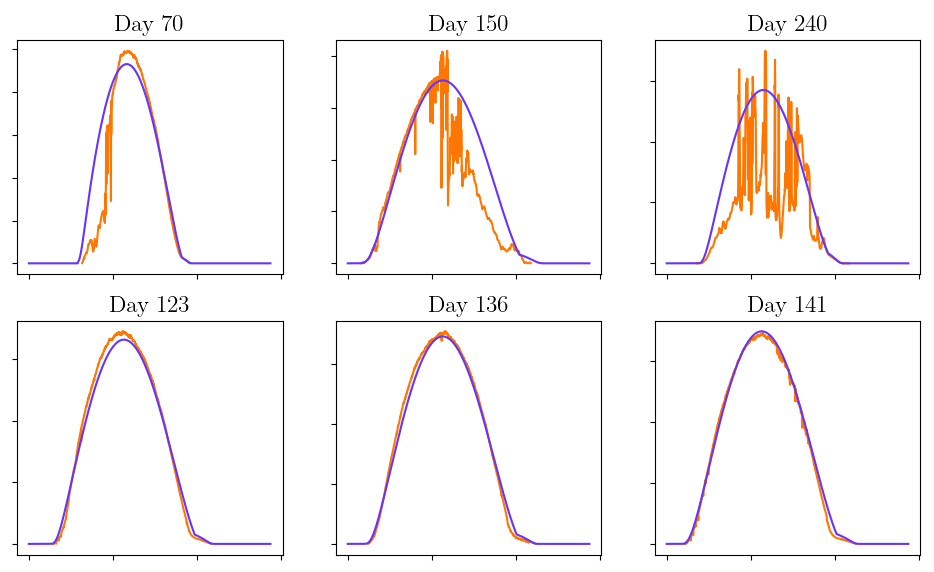
\includegraphics[width=1\linewidth]{pics/multiday_vs_neat}
\figcaption{Power output of FMI Kumpula PV installation and the pvlib POA simulation computed with the parameters \ref{table_fmi_helsinki_kuopio_parameters}. Horizontal axis on the graphs corresponds to time and vertical axis marks the estimated power values. The purpose of the graphs is to display the different shapes and deviations from POA models and thus axis names and numbers were left out. Upper row contains randomly selected days while as the lower row has days chosen by a clear sky algorithm mentioned in chapter \ref{clearskyalgo_chapter}. Measurements are from 2017. POA irradiance values were multiplied by 20 in order to match the curves values on power axis.}
\label{fig-multidaypoavsmeasurements}
\end{figure}



% On the 70th and 150th day, the first and last minutes do not seem to be exactly the same as in the simulation, but the difference seems minor and it is occuring in different directions.






%\textit{The following claims are unverified conjectures, but the smooth shape and the early date of the first graph could hint that the increased peak production on the 70th day could be due to reflections from snow, while as the more irregular production on the 150th and 240th day would seem to indicate that the variation is caused by clouds. Filtering out days such as the 150th or the 240th from the dataset should be rather simple as the high frequency component is noticeable, but low frequency deviations such as the smooth increase in production of the 70th day could prove to be more difficult to detect algorithmicly.}






\newpage
\newpage
\newpage
\section{Influence of different parameters on the PVlib poa model}
\label{influence_parameters}
%In order to use the POA model for solving system parameters, each model parameter should 


%the plane of array irradiance function parameters should all have an unique relationship with the 


% the parameters of the POA simulations have to be independent. This means that two different points in the parameter space should not result in the same POA curve as if this occurs, it will not be possible to determine 



%This means that when two different inputs are given to the PVlib plane of array irradiance function, the outputs should never be the same. As 






%In simplified terms, this independence means that no two sets of different parameter should result in the same POA curve, however this property of sameness fairly challenging to measure in a meaningful way due to the complex nature of the POA curves. %Methods for evaluating this difference are still needed as otherwise it would not be possible to mathematically prove that the a POA simulation with certain parameters is a better fit to the measurements than a POA simulation with different parameters.






%The two approaches used in this thesis are significant point differences and area difference. In significant point based difference measurements, a set of sigificant points are chosen from the plots. These could be the peak or last/first minute 


\begin{figure}[ht!]
\centering
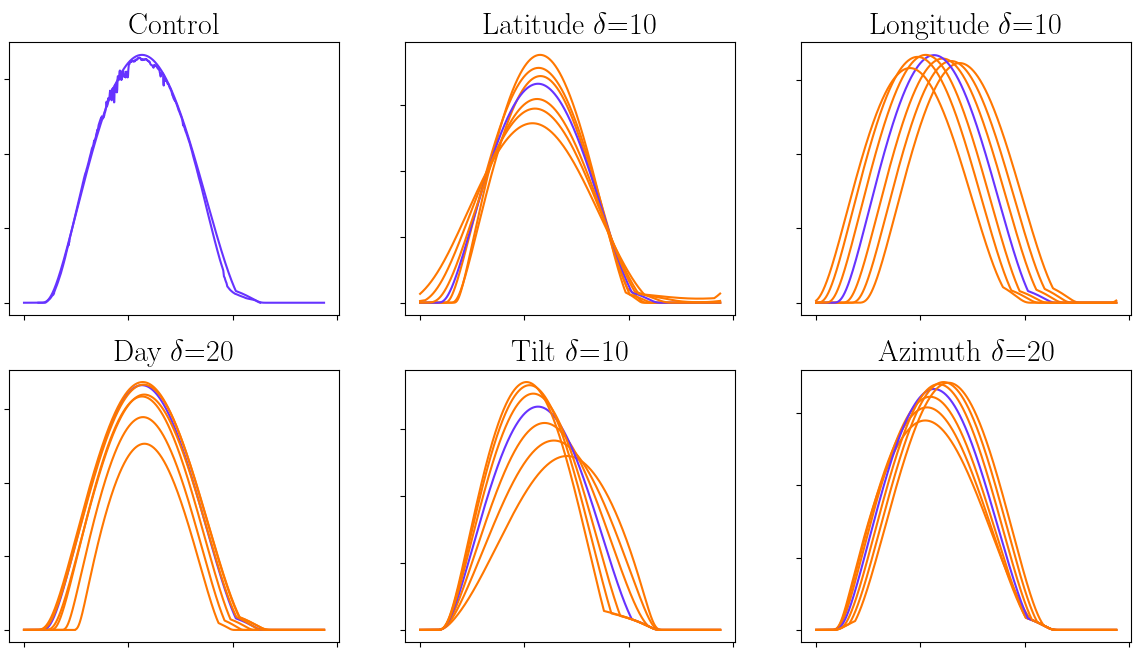
\includegraphics[width=0.8\linewidth]{pics/poa_eval_new_crop}
\figcaption{Influence of changes in PVlib simulation parameters on generated power output curves. Control shows FMI Helsinki measurements and simulation with the same parameters as the Helsinki installation. Simulated power values are multiplied by 19 in order to match values on y-axis.}
\label{fig_poa_different_parameters}
\end{figure}

\noindent In the best case scenario each of the simulation function inputs would affect one measureable property in the irradiance plots and their relationship would be bijective. To give an example, if the peak power minute was isolated from all other parameters than the longitude and the relationship between longitude and peak power minute was linear, it would be possible to solve the peak power minute to longitude function with just a few plane of array irradiance simulations.

In the exact opposite case where every measureable property of irradiance plots is affected by every input parameter, solving the parameters would be much harder or even impossible. For example if all of the parameters influenced the same traits to different extents and the system was not bijective, multiple parameter combinations could result in the same simulated power graph. In a such system there would not be a single solution but rather a set of possible solutions.

The problem of solving installation parameters lies somewhere in between the two extremes. The longitude parameter would seem to shift the curve along the time axis where as tilt and azimuth parameters do not affect the first or last non-zero minutes but they do affect the shape of the curve. Observations of parameter to trait interactions are listed on table \ref{table_traits}.



\begin{table}[H]
\centering
\begin{tabular}{r|cc} \hline\hline

 Parameter & Traits affected\\ \hline
 Latitude & Shape, first and last minute times\\
 Longitude & First and last minute times\\
 Tilt & Shape\\
 Azimuth & Shape\\

\hline\hline
\end{tabular}
\tabcaption{Function input to observed trait table.}
\label{table_traits}
\end{table}


%Base on these observations, the relationship between longitude and the First and last minute times would seem like the best starting point for parameter solving.

%If the POA model is assumed to be accurate, the model could be used to simulate the effects of different parameters on power generation. This could provide insights into the relationship between patterns in the data and the parameters of the system. The relevant parameters to simulate and their default values can be seen in table \ref{table_default_parameters_poa_simulations}. In the following simulations, only one of the default parameters is varied. This is done in order to isolate the effect of individual parameters.



%\begin{table}[!ht]
%\centering
%\begin{tabular}{r|c} \hline\hline

% Parameter & Value \\ \hline
% Day & $180$  \\
% Latitude & $60^\circ$  \\
% Longitude & $28^\circ$  \\
% Panel tilt & $30^\circ$ \\
% Panel angle & $180^\circ$  \\
%\hline\hline
%\end{tabular}
%\tabcaption{Default parameters for POA simulation used in this section. }
%\label{table_default_parameters_poa_simulations}
%\end{table}


\newpage

\subsection{Influence of different longitudes}
\label{section_different_longitudes}

\begin{figure}[ht!]
\centering
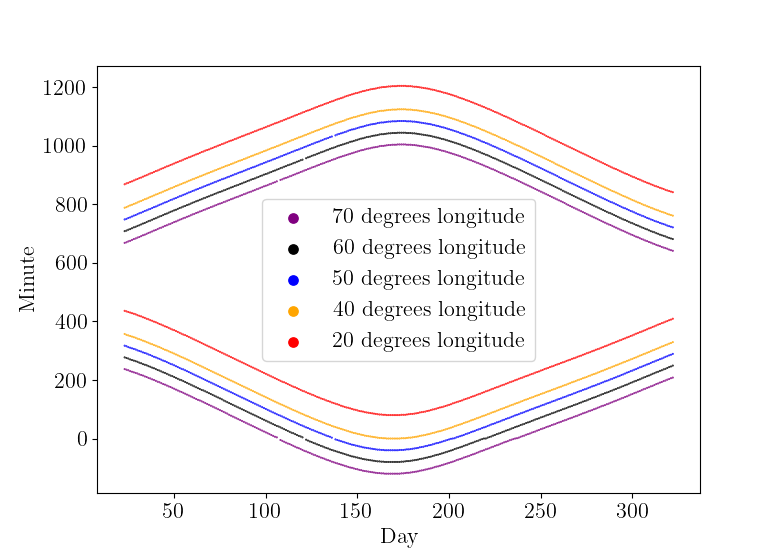
\includegraphics[width=1\linewidth]{pics/poa_var_lon}
\figcaption{First and last non-zero minutes of each day from year long simulations at different longitudes.}
\label{fig-poa_var_lon2}
\end{figure}

\noindent Based on earlier observations listed in table \ref{table_traits}, solving the longitude of installations would seem like a sensible starting point. The figure comparing the effects of different parameters seemed to suggest that the relationship between longitude and significant minute times is very close to linear and the same is seen here in figure \ref{fig-poa_var_lon2}. In Hagdadi 2017 \cite{navid_australian_article} and in Williams 2012 \cite{older_solar_solver_article} this relationship was used in order to determine the geographic longitude. The algorithms used by both of the articles relies on calculating an approximation for the time of the solar noon based on the average of the first and last minutes, this solar noon minute is then translated into a geographic longitude coordinate.



%There are at least two ways of estimating the longitude from the UTC solar noon time. First method is based on fitting a linear equation to a list of known solar noon to longitude-pairs. This would result in an equation of the form $f(x) = 0.25^\circ* x + b$ where the solar noon minute $x$ is multiplied by the constant $0.25$. The constant of $0.25^\circ$ comes from dividing a full circle by the amount of minutes in a day, 1440. The constant $b$ is around $-180^\circ$ and it is the result of solar noon occuring close to noon.
%In the figure \ref{fig-poa_var_lon2}, the relationship between the first and last minutes of a day and the geographic longitude can be seen to be linear. This linear equation should be of the form $f(x) = 0.25^\circ* x + b$ where the solar noon minute $x$ is multiplied by the constant $0.25$. The constant of$0.25^\circ$ comes from dividing a full circle by the amount of minutes in a day, 1440. The constant $b$ is roughly $-180$ degrees as that is the offset required for adjusting solar noon from



%and the figure \ref{fig-poa_var_lon2} it would seem that the relationship between longitudes and first and last minutes is a good starting point for parameter so


%at least very close to linear. In Hagdadi 2017 \cite{navid_australian_article} and in Williams 2012 \cite{older_solar_solver_article} this relationship was used in order to determine the geographic longitude. The algorithms used by both of the articles relies on calculating an approximation for the time of the solar noon based on the average of the first and last minutes, this solar noon minute is then translated into a geographic longitude coordinate.

% and a similar algorithm is detailed in []..




\newpage

\subsection{Influence of different latitudes}
\label{section_different_latitudes}

\begin{figure}[ht!]
\centering
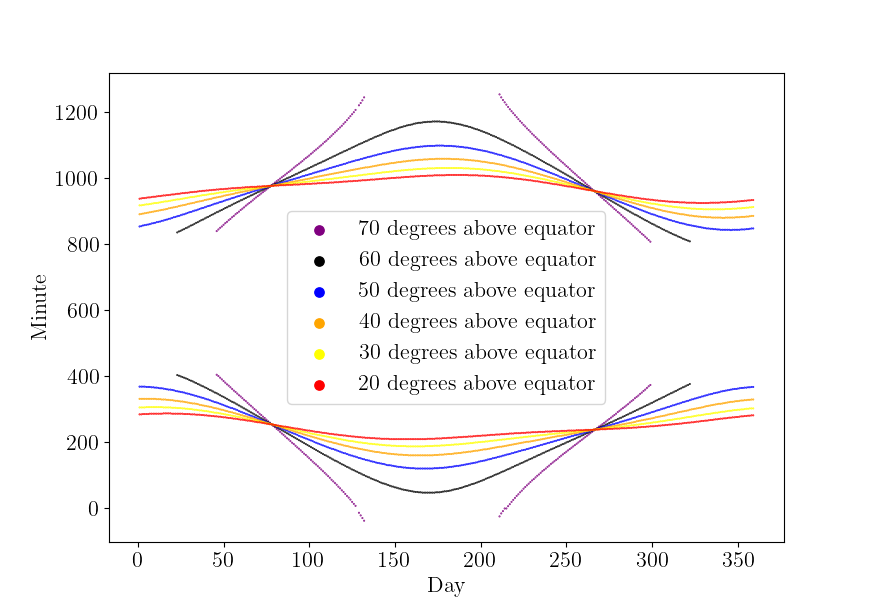
\includegraphics[width=1\linewidth]{pics/poa_var_lat}
\figcaption{First and last non-zero power minutes of each day from year long simulations at different latitudes}
\label{fig_poa_var_lat}
\end{figure}

\noindent The latitude simulations show that the day length stays fairly consistent for locations close to the equator, but with latitudes of $50^\circ$ and higher, the day to day variation is significant. These POA simulations would imply that the region around equinoxes to be ideal for day length based analysis as there day length is always well defined and the rate of change can be measured. 


\newpage

\section{Increasing accuracy of solar PV simulations}
\label{section_increased_accuracy_simulations}

\begin{figure}[h]
\centering
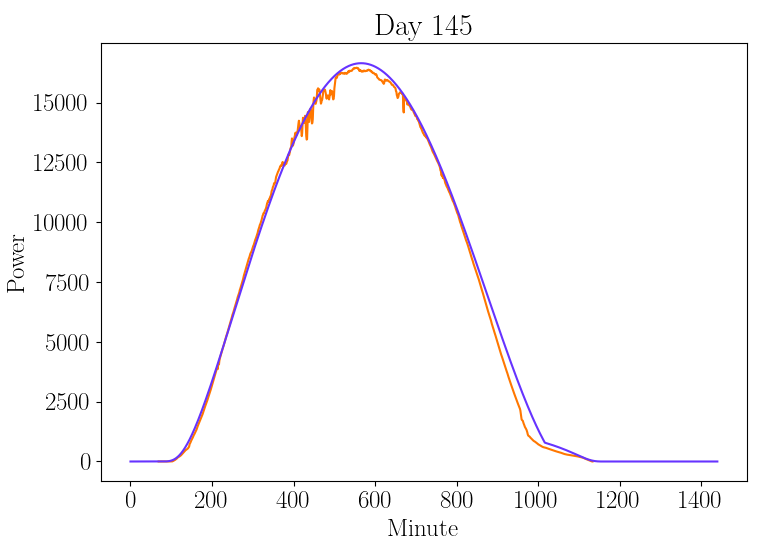
\includegraphics[width=0.7\linewidth]{pics/poa_eval_single_day}
\figcaption{Figure displaying deviations between simulated values and measured values.}
\label{fig-poa_eval_single_day}
\end{figure}

\noindent Figure \ref{fig-poa_eval_single_day} show that simulations are fairly accurate but there seems to be some deviations between the simulated values and the measurements. The two significant deviations are the noise during peak power generation period and the smooth decrease in power generation during the last hours of the day. The peak power generation noise is likely to be caused by decreases in efficiency due to heat the occasional cooling from gusts of wind. The second deviation between the model and actual measurements is likely to be caused by panel reflections as the south-east orientation of the solar panels results in a high angle of incidence during the last hours of the day.

Modeling these physical phenomena is possible to an extent if the components of plane of array irradiance are used instead of the POA values. As per Sandia National Laboratories \cite{sandia_poa}, the three components of plane of array irradiance are direct normal irradiance(DNI), global horizontal irradiance(GHI) and diffuse horizontal irradiance DHI. A physically accurate model would compute the absorbed radiation by first projecting the irradiance components to the plane of array adn the estimating the losses caused by reflections. After this is accomplished, the absorbed irradiance could be used to estimate panel temperature and power output.









\chapter{Estimating geographic location}
\label{chapter_est_geoloc}
In order to evaluate the performance of longitude and latitude estimation functions, it may prove useful to be able to translate the error values from degrees to kilometers. The following two equations \ref{equation_latitude_delta_km} and \ref{equation_longitude_delta_km} can be used to approximate the degree deltas of longitude and latitude estimation functions in kilometers. Note that these functions can be off by several percents as they rely on the assumption that the Earth is a perfect sphere and not an irregular ellipsoid.


\hfill \break
%%%%%%%%%%%%%%%%%%%%%%%%%%%%%%%%%%%%%%%%%%%%%%%%%%%%%%%%%%%%%%%%%%%%% START
\noindent\textbf{Latitudinal distance to kilometers}(Distance on North-South axis)
%
\begin{equation}
\begin{split}
\label{equation_latitude_delta_km}
Distance_{latitudinal}(lat\_d)=(40 000km/360^\circ)* lat\_d
\end{split}
\end{equation}

\noindent Where $lat\_d$ is the distance between two points in degrees latitude and 40000km is an approximation for Earths circumference.

\vspace{5mm} %5mm vertical space
%%%%%%%%%%%%%%%%%%%%%%%%%%%%%%%%%%%%%%%%%%%%%%%%%%%%%%%%%%%%%%%%%%%%% END

%%%%%%%%%%%%%%%%%%%%%%%%%%%%%%%%%%%%%%%%%%%%%%%%%%%%%%%%%%%%%%%%%%%%% START
\noindent\textbf{Longitudinal distance to kilometers at given latitude}(Distance on East-West axis)
%
\begin{equation}
\begin{split}
\label{equation_longitude_delta_km}
Distance_{longitudinal}(lon\_d, lat)=(40 000km/360^\circ)* cos(lat)*lon\_d
\end{split}
\end{equation}

\noindent Where $lon\_d$ is the distance in degrees longitude and $lat$ is the latitude for which the distance is calculated.



\vspace{5mm} %5mm vertical space

\noindent As long as the deviations are not significant and highly accurate error values are not needed, the total error in absolute terms can be estimated by using the latitudinal and longitudinal distances as the x and y coordinates on a cartesian plane and computing the euclidean distance between the origin and resulting point.

%%%%%%%%%%%%%%%%%%%%%%%%%%%%%%%%%%%%%%%%%%%%%%%%%%%%%%%%%%%%%%%%%%%%% END

\newpage
\section{Estimating geographic longitude}
\noindent As mentioned in sections \ref{section_different_latitudes} and \ref{section_different_longitudes}, the geographic location of a PV system has a strong connection to the timing of the first and last non-zero measurements of each day whereas the influence of tilt and facing parameters seems to be nonexistent. The relationship would seem to be so clear that without further analysis it would be tempting to use fairly simplistic mathematical models for these estimations. The following longitude estimation function \ref{equation_naive_longitude} can be derived with the use of two basic assumptions. These ssumptions are that solar noon occurs at 12:00 or 720 minutes at longitude 0 each day and at 6:00 or 360 minutes at 90 degrees. Rest of the values can then be linearly interpolated. Note that here solar noon refers to the midpoint between the first and last non-zero minute which is different from astronomical solar noon which occurs nearly at the same time.

\hfill \break


%The simpler of these relationships is the relationship between the longitude and first and last non-zero minute times. Based on the figure \ref{fig-poa_var_lon2}, this relationship seems to be very close to linear. This makes the use of a simple linear equation rather compelling. 



%%%%%%%%%%%%%%%%%%%%%%%%%%%%%%%%%%%%%%%%%%%%%%%%%%%%%%%%%%%%%%%%%%%%% START

\noindent\textbf{Naive solar noon to longitude equation}
%
\begin{equation}
\begin{split}
\label{equation_naive_longitude}
Longitude(sn)=180^\circ-\frac{360^\circ}{1440}*sn
\end{split}
\end{equation}
Where $sn$ is the approximated solar noon minute calculated by taking the average of first and last non-zero power generation minute of a day. % $0.25$ or $360/1440$ corresponds to the longitude degrees per minute and $180$ is used as offset value. This naive equation assumes that solar noon occurs at 12:00 or 720 minutes each day at $0^\circ$ longitude. Note that here solar noon refers to the midpoint between the first and last non-zero minute which is different from astronomical solar noon which occurs nearly at the same time.

\hfill \break
%%%%%%%%%%%%%%%%%%%%%%%%%%%%%%%%%%%%%%%%%%%%%%%%%%%%%%%%%%%%%%%%%%%%% END


\noindent The simplicity of \ref{equation_naive_longitude} makes the equation appealing, but the assumption of solar noon occuring at 720 minutes should still be verified. In figure \ref{fig_solarnoons} solar noons can be seen to occur at around 720 minutes at longitude 0 but they can also be observed occuring 15 minutes earlier or later than that. This 15 minute delta would translate into an error range of $\pm 3.75$ degrees or approximately $\pm 200 km$ at the latitudes of Helsinki according to the equation \ref{equation_latitude_delta_km}.

\begin{figure}[ht!]
\centering
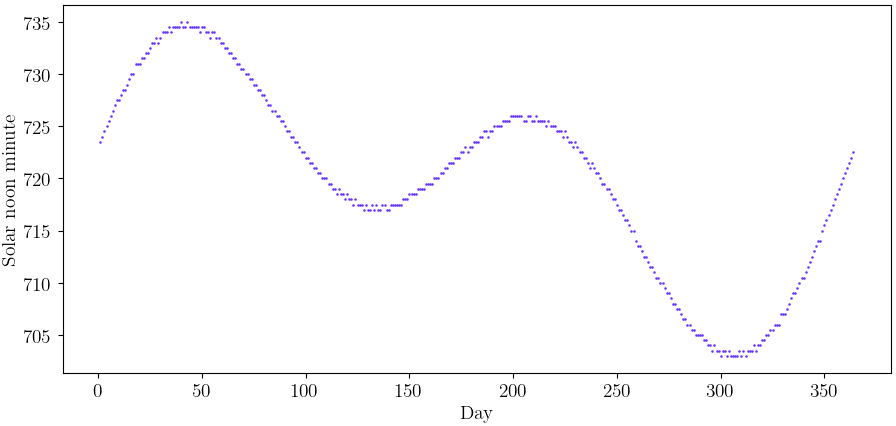
\includegraphics[width=1\linewidth]{pics/solarnoons2}
\figcaption{Approximations of solar noon minutes based on PVlib POA function at longitude $0^\circ$ for year 2023. This pattern is caused by the Earths axial tilt and elliptical orbit around the Sun \cite{solarnoonpattern}.}
\label{fig_solarnoons}
\end{figure}



Knowing that the PV installation is within a 400 kilometer wide slice should be in most cases be accurate enough for determining the country in which the PV installation is located in, but for most other purposes this level of accuracy is unlikely to be valuable. Fortunately the naive model can be improved upon by taking the solar noon timing variation into account. \hfill \break


\newpage
%%%%%%%%%%%%%%%%%%%%%%%%%%%%%%%%%%%%%%%%%%%%%%%%%%%%%%%%%%%%%%%%%%%%% START
\noindent\textbf{Improved longitude estimation function }
%
\begin{equation}
\begin{split}
\label{equation_longitude_estimation_2}
Longitude(sn)= \frac{360}{1440}(sn_{poa}-sn)
\end{split}
\end{equation}

\noindent Where $sn$ is the solar noon estimate based on measurement data and $sn_{poa}$ is the simulated solar noon at 0 degrees longitude. The new function parameter $sn_{poa}$ compensates for the variation seen in \ref{fig_solarnoons}.


%%%%%%%%%%%%%%%%%%%%%%%%%%%%%%%%%%%%%%%%%%%%%%%%%%%%%%%%%%%%%%%%%%%%% END

\vspace{5mm}


\noindent
%The improved function \ref{equation_longitude_estimation_2} should be much more accurate than the earlier longitude function. as the errors in estimates should primarily be the result of bias in the measurements data.


%In figure \ref{fig_solarnoons_poa_vs_measurement} the solar noon estimates calculated by taking the average of first and last non-zero minute of the day can be seen to preceed the solar noons by roughly 8 minutes. This systematic bias could be explained by the east facing orientation of the panels and correcting for the bias could could be fairly difficult. 

\vspace{0.5cm}
%The theoretical accuracy at this stage could be as high as $\frac{360^\circ}{1440} = 0.25^\circ$ but 
\noindent The improved algorithm should no longer have a systematic error of up to 15 minutes after the analemma has been taken into account. In addition to correcting for the irregular solar noon timing, the algorithm can be improved even further by using the algorithm on larger sections of data and averaging the results, or alternatively the algorithm could be applied only on selected cloud free days where the expected errors are likely to be smaller. If the unfiltered multi-day approach is used, choosing the right day range is crucial. If the range is too narrow, a single outlier value can distort the results significantly, however if the whole year is used, certain periods of the year may contain more noise than others and thus their use could decrease the accuracy of the results. The two scatterplots in figure \ref{fig_first_last_kuopio_helsinki} show that the data quality from the very first and last days of the year seem to be significantly worse than the data from the longest days of the year. The same graph would also seem to suggest that overall data quality decreases the further north the installation is. Based on these visualizations, days outside the range of 100th to 280th would seem unsuitable for first and last minute based analysis between latitudes $60^\circ N$ and $63^\circ N$. 

%noise present in power generation measurements may result in significant errors in estimates based on individual days. These errors can be mitigated by using the algorithm on larger sections of data and averaging the results, or alternatively the algorithm could be applied only on selected cloud free days where the expected errors are likely to be smaller. If the unfiltered multi-day approach is used, choosing the right day range is crucial. If the range is too narrow, a single outlier value can distort the results significantly, however if the whole year is used, certain periods of the year may contain more noise than others and thus their use could decrease the accuracy of the results. The two scatterplots in figure \ref{fig_first_last_kuopio_helsinki} show that the data quality from the very first and last days of the year seem to be significantly worse than the data from the longest days of the year. The same graph would also seem to suggest that overall data quality decreases the further north the installation is. Based on these visualizations, days outside the range of 100th to 280th would seem unsuitable for first and last minute based analysis between latitudes $60^\circ N$ and $63^\circ N$.


\begin{figure}[ht!]
\centering
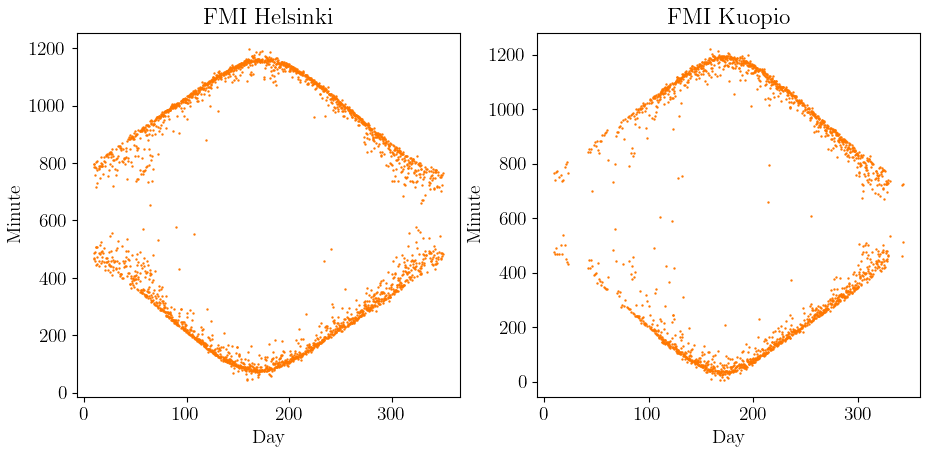
\includegraphics[width=1\linewidth]{pics/first_last_helsinki_kuopio2}
\figcaption{First and last non-zero power minutes of each day during years 2017 to 2021 from FMI Helsinki and Kuopio datsets.}
\label{fig_first_last_kuopio_helsinki}
\end{figure}



\subsection{Longitude estimation results}
The improved algorihm was tested on the day range of 125th to 250th of each year from both FMI datasets and the results can be seen on the table \ref{table_geolocator_results}. For the Helsinki installations these estimates are all off by less than $0.3^\circ$ while as the Kuopio installation deltas are a bit higher with max of just over $1^\circ$. More impressively, the mean delta of multiple years for the Helsinki dataset is just $0.07^\circ$ and $0.457^\circ$ for Kuopio. In kilometers, the mean deltas can be approximated to 4 and 28 kilometers respectively. The lower accuracy of the Kuopio estimations could be due to multitude of factors ranging from differences in local climate or lower elevation of the installation among others. 




%as seen from the earlier figure \ref{fig_multiyear_first_last}, even the best sections in the dataset still have a fair bit of noise. This noise can be averaged out to some extent by performing the longitude estimations on multi-day sections and then averaging the results. The same figure suggests that the data quality is highest during the middle of the year and so the range of 125th to 250th day was chosen for the following computations. The following table \ref{table_geolocator_results} shows the results of multi-day longitude estimations for both Helsinki and Kuopio FMI PV installations. 



\begin{table}%[!h]
\centering
\begin{tabular}{r|c|c|c|c} \hline\hline

 Year & Longitude Helsinki & $\Delta^\circ$  & Longitude Kuopio & $\Delta^\circ$ \\ \hline
 2021 & $25.115^\circ$  & $0.154^\circ $  & $26.625^\circ$ & $-1.009^\circ $ \\
 2020 & $25.029^\circ$ & $0.068^\circ $& $27.691^\circ$  & $0.057^\circ $ \\
 2019 & $24.944^\circ$ & $-0.017^\circ $& $27.411^\circ$ & $-0.223^\circ $  \\
 2018 & $25.243^\circ$ & $0.282^\circ $& $26.862^\circ$ & $-0.772^\circ $ \\
 2017 & $24.836^\circ$  & $-0.125^\circ $& $27.297^\circ$ & $-0.337^\circ $ \\
 mean & $25.031^\circ$  & $0.07^\circ $& $27.177^\circ$ & $-0.457^\circ $ \\
\hline\hline
\end{tabular}
\tabcaption{Means of multi-day longitude estimations from 125th to 250th day of each year.}
\label{table_geolocator_results}
\end{table}

\newpage
\subsection{Possible issues and further development ideas}
While experimenting with the solar minute estimation functions, a curious trait was found. In figure \ref{fig_solarnoontimes}, the average of the first and last minute is approximately the same at different latitudes as long as the latitude is below 50 degrees. As the latitude is increased, the solar noon estimates begin to deviate significantly, becoming strongly skewed after 70 degrees. At first this behavior seems strange as astronomical solar noon should occur happen at the same time when longitude and the day are the same regardless of latitude. However as the solar noon estimates are calculated based on the first and last non-zero irradiance minute of the day, it would make sense that the estimations could be off by significant amount during equinoxes due to rapid changes in day lengths. Figuring out how significantly this affects longitude estimations is challenging. In theory, if the same bias occurs in both the measurements and the model, no corrections would be needed. The effect should be also lessened by using longer day ranges for predicting longitudes or by making sure that the intervals include an equal amount of days from both halves of the year. 

Improvements in the algorithm accuracy could also be achieved via by increasing the sampling interval of the irradiance simulations. PVlib POA simulations include a parameter for sampling frequency which is currently set to 1-per-minute in order to match the measuring frequency of FMI datasets. This could be increased to 1-per-second and the added resolution could help in determining more accurate estimates for solar noon times, resulting in possible gains in algorithm accuracy. 




\begin{figure}[]
\centering
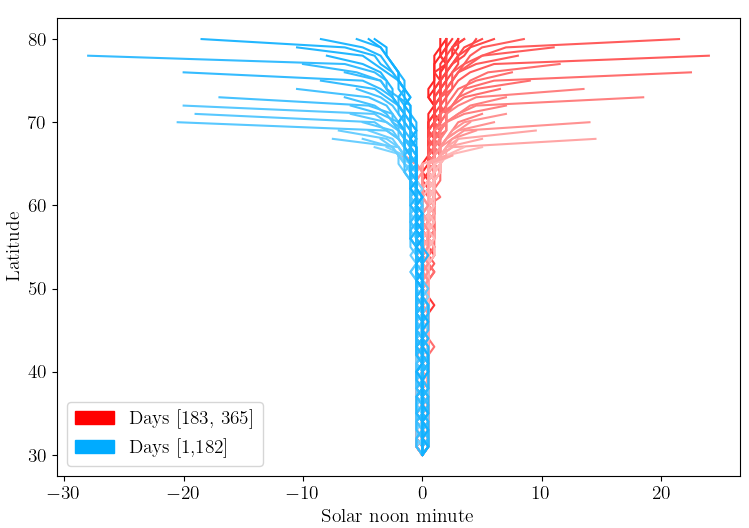
\includegraphics[width=1\linewidth]{pics/solarnoontimes2}
\figcaption{Relationship between latitude parameter and estimated solar noon time. Each line represents a different day of the year and x-axis values are normalized so that each line begins at 0 deviation. Lines with darker colors mark days which are further away from spring and fall equinoxes.}
\label{fig_solarnoontimes}
\end{figure}







%\textbf{Longitude estimation notes}

\newpage 
\section{Estimating geographic latitude}
Similarly to the longitude, the latitude of an installation is strongly connected to the timing of the first and last non-zero minutes of the day. In figure \ref{fig_poa_var_lat}, the simulated first and last minutes can be seen to change day by day at varying rates based on the latitude. In mathematical terms it could be said that the derivative of the day-to-first-minute function is determined by the latitude of the installation. And for the days around equinoxes, and at higher latitudes of $50^\circ$ to $70^\circ$, this relationship would seem to be bijective as per earlier figure \ref{fig_poa_var_lat}. Based on these observatyions, the obvious method for solving latitudes would be the following algorithm. \hfill


\subsection{Latitude algorithm}
%\noindent\textbf{Latitude algorithm}
\begin{enumerate}
  \item Simulate first non-zero minutes over a specific day range at latitude $l$.
  
  \item Fit a linear equation to the simulated day to first minute pairs from step 1.
  
  \item Repeat steps 1 and 2 for every relevant latitude, graph linear equation slopes from step 2 as X-axis values and latitudes as Y axis values.
 
  \item Fit an n-degree polynomial equation to the graph from step 3.
  
  \item If the day length change can be inferred from PV installation power output, this rate of change can then be used as the input for the polynomial from step 4 and the value of the polynomial should be the geographic latitude.
\end{enumerate}

\noindent
\textbf{Notes:}
%A visualization of the algorithm can be seen in the following figure \ref{fig_slope_to_latitude}. 
Due to seasonal differences in data quality, polar winters and the midnight sun, the range of days chosen for the algorithm is important. If the range is short, individual outliers in measurements can result in large errors. Whereas if the range is too long, it will be harder to choose the range while avoiding low data quality sections. In the algorithm visualization figure \ref{fig_slope_to_latitude}, the range of 250th to 300th seems to result in acceptable slope to latitude curve smoothness.
\newpage
\subsection{Latitude algorithm visualization}
\begin{figure}[ht!]
\centering
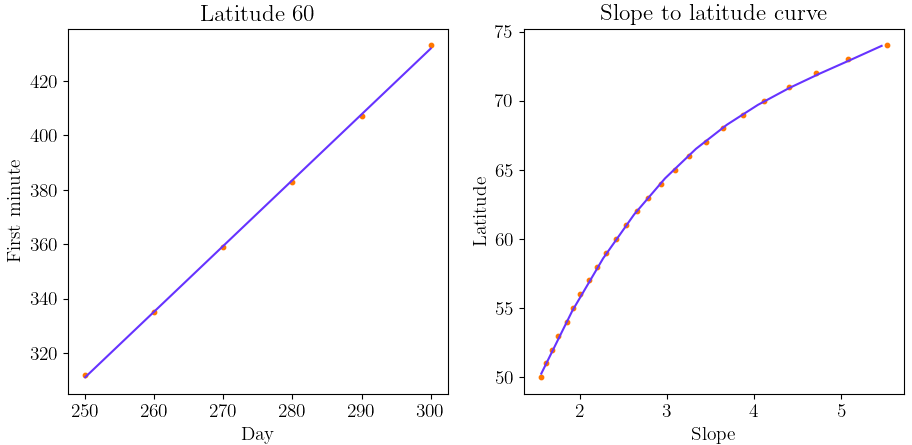
\includegraphics[width=1\linewidth]{pics/slope_to_latitude3}
\figcaption{Graph on the left shows the almost linear relationship between day and simulated first minutes. Second graph shows the relationship between the slope angle and latitude.}



%the latitude algorithm steps 1 and 2 for day range 250 to 300 at latitude 60 and the linear model fitting. Second graph shows steps 3 and 4 in which slope angles are plotted agains latitudes. The fitted 3rd degree polynomial is $f(x)= 0.305x^3 - 4.607x^2 + 25.953x + 19.908$.}
\label{fig_slope_to_latitude}
\end{figure}



\begin{table}[!ht]
\centering
\begin{tabular}{r|c|c} \hline\hline
 \multicolumn{3}{ c }{FMI Kumpula}\\\hline
Year & Predicted latitude & Error\\
2021 & $61.365^\circ$ &  $1.161^\circ$\\
2020 & $64.493^\circ$ &  $4.289^\circ$\\
2019 & $63.121^\circ$ & $2.917^\circ$\\
2018 & $61.190^\circ$ & $0.986^\circ$\\
2017 & $57.515^\circ$ & $-2.789^\circ$\\


\hline\hline
\end{tabular}
\tabcaption{Results from estimating the latitude of FMI Kumpula PV installation with the preceeding algorithm. Day range of 250th to 300th was used.}
\label{table_geolocator_latitude_results}
\end{table}
\vspace{3mm}
\noindent

\subsection{Improving the algorithm}
The results of the algorithm shown in table \ref{table_geolocator_latitude_results} are somewhere in the correct range, but the delta of over $4^\circ$ in the 2020 estimate is significant and much higher than the error of the longitude estimation algorithm. The first step in improving the algorithm would be the use of last non-zero days as well as the first non-zero days. This doubles the amount of outputs from the algorithm and while doubling the amount of outputs does not directly increase the accuracy of the algorithm, it can provide additional insights into the performance of the algorithm. This is especially valuable as the available datasets are small.



\begin{table}[!ht]
\centering
\begin{tabular}{r|c|c|c|c} \hline\hline

\multicolumn{5}{ c }{FMI Kumpula}\\\hline
Year & First min. p. & Error &  Last min. p. & Error \\
2021 & $61.365^\circ$ &  $1.161^\circ$ & $63.685^\circ$ & $3.481^\circ$\\
2020 & $64.493^\circ$ &  $4.289^\circ$ & $64.288^\circ$ & $4.084^\circ$\\
2019 & $63.121^\circ$ & $2.917^\circ$ & $66.762^\circ$ & $6.558^\circ$\\
2018 & $61.190^\circ$ & $0.986^\circ$ & $60.230^\circ$ & $0.026^\circ$\\
2017 & $57.515^\circ$ & $-2.789^\circ$  & $62.256^\circ$ & $2.052^\circ$\\

\hline\hline
\end{tabular}
\tabcaption{Latitude algorithm with added output for last minutes based prediction.}
\label{table_geolocator_latitude_results_f_and_l}
\end{table}


%Figure \ref{table_geolocator_latitude_results_f_and_l} shows that predictions based on first and last minutes contain similar errors. This is to be expected and it shows that both first and last minutes of each day have similar potetial for latitude estimation. 


The second step in improving the algorithm is choosing the best possible day range for latitude estimation. One way of choosing the day ranges would be by testing multiple day ranges and choosing the range which results in the lowest average absolute error from the known latitude. While this would result in a circular proof, by using multiple datasets from different geographic regions, the method could be used to find universally well behaving day ranges which could then be used for datasets with unverified or unknown coordinates.

\textit{Standard deviation minimization} is the second option for automated day range selection. As there are two estimated latitude values per year, datasets with $n$ years of data would provide $n*2$ estimated latitude values. Standard deviation of these values could expected to be small if the day interval does not contain days with bad data quality and this means that the interval selection can be automated. However exhaustively searching the day interval space with reasonable intervals can be slow and as seen in the figure \ref{fig_heatmap3d2}, low standard deviation intervals are common in the parameter space. As a result, an arbitrarily chosen long interval is likely to perform almost as well as the very best algoritmicly chosen interval.

%This same figure indicates that an arbitrarily chosen long interval is likely to perform almost as well as the very best algoritmicly chosen interval.


%If the day range is selected well, these estimations could be expected to be tightly grouped. This tight grouping can be measured by calculating the standard deviation and thus the day interval with the lowest standard deviation could be expected to result in the best latitude estimation. A such method relies on the assumption that low standard deviation correlates with good preditions, but this assumption can be shown to be false or missleading. The following figure \ref{fig_heatmap3d2} shows that 

\begin{figure}[]
\centering
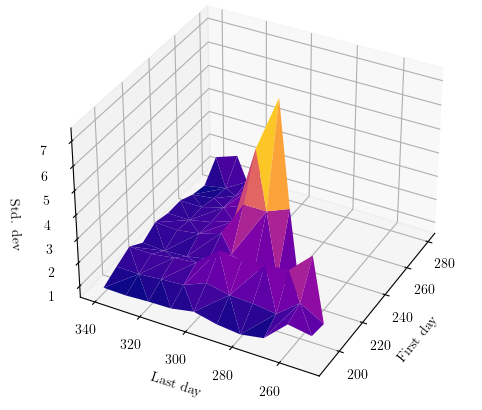
\includegraphics[width=0.5\linewidth]{pics/heatmap3d2}
\figcaption{3D -surface where X and Y -axis correspond to the interval star and end days and Z -axis marks the standard deviation of latitude estimations when the interval is used to predict latitudes from FMI Kuopio dataset.}
\label{fig_heatmap3d2}
\end{figure}

\newpage

\subsection{Latitude estimation results}
The following two tables contain examples of the results of the latitude estimation algorithm. Results of the latitude estimation algorithm are not as good as the longitude estimations, but for now they will suffice. The predictions follow a similar patter as the previous longitude estimations in that predictions for the Helsinki installation are grouped tighter and their errors are lower than those of the Kuopio installation. 

\begin{table}[!ht]
\centering
\begin{tabular}{r|c|c|c|c} \hline\hline

\multicolumn{5}{ c }{FMI Helsinki latitude estimation results}\\\hline
Year & First min. p. & Error &  Last min. p. & Error \\

2021 & $59.792^\circ$ &  $-0.677^\circ$ & $60.186^\circ$ & $-0.334^\circ$\\
2020 & $59.792^\circ$ &  $-0.412^\circ$ & $60.186^\circ$ & $-0.018^\circ$\\
2019 & $59.896^\circ$ & $-0.308^\circ$ & $59.558^\circ$ & $-0.646^\circ$\\
2018 & $59.945^\circ$ & $-0.259^\circ$ & $59.463^\circ$ & $-0.741^\circ$\\
2017 & $60.577^\circ$ & $0.373^\circ$  & $60.008^\circ$ & $-0.196^\circ$\\

\hline\hline
\end{tabular}
\tabcaption{Estimated latitudes for FMI Helsinki Kumpula dataset with day range of 190th to 250th}
\label{table_geolocator_latitude_results_f_and_l2}
\end{table}

\begin{table}[!ht]
\centering
\begin{tabular}{r|c|c|c|c} \hline\hline

\multicolumn{5}{ c }{FMI Kuopio latitude estimation results}\\\hline
Year & First min. p. & Error &  Last min. p. & Error \\
2021 & $62.626^\circ$ &  $-0.266^\circ$ & $63.197^\circ$ & $0.305^\circ$\\
2020 & $62.259^\circ$ &  $-0.633^\circ$ & $61.895^\circ$ & $-0.997^\circ$\\
2019 & $62.983^\circ$ & $0.091^\circ$ & $62.708^\circ$ & $-0.184^\circ$\\
2018 & $62.722^\circ$ & $-0.170^\circ$ & $62.874^\circ$ & $-0.018^\circ$\\
2017 & $61.669^\circ$ & $-1.223^\circ$  & $61.152^\circ$ & $-1.740^\circ$\\

\hline\hline
\end{tabular}
\tabcaption{Estimated latitudes for FMI Kuopio Kumpula dataset with day range of 190th to 280th.}
\label{table_geolocator_latitude_results_kuopio}
\end{table}

\subsection{Possible issues and further development ideas}
PVlib POA based first and last minute estimations are slow to compute and thus exhaustively searching the day interval space can take up to several hours of computing time. As only the first and last minute times are needed, the use of simpler computational methods could improve the computation speed significantly, allowing for the use of brute force day range selection algorithms.

Different methods could also be used. In Hagdadi 2017 \cite{navid_australian_article} latitude estimations are done by fitting solar irradiance models with 3 unknown parameters to power generation measurement data. The latitude deltas of 1.65 to 3.42 degrees in the 2017 article are higher than those achieved in this thesis, however as the datasets, geographical regions and algorithms are different, direct comparison can not be made.

%by this paper, however as the datasets, geographical regions and algorithms are different, direct comparison can not be made.

In earlier figure \ref{fig_slope_to_latitude} the slope to latitude fitting can be seen to be slightly off. This is because the polynomial used is of 2nd degree and higher degree polynomials may result in a closer fit. Similarly a piecewise linear interpolation based fitting could result in a more accurate model and thus better estimation accuracy.


\newpage
\section{Combined latitude and longitude estimations}
As it is unlikely that the longitude and latitude estimation algorithms are used in isolation from one another, their results should be examined together. This can be done by plotting the estimated locations on a map. Here the two installations in Helsinki and Kuopio and their predicted locations per year are plotted side by side with day range of 190 to 280.

\begin{figure}[h]
	
     \centering
     \begin{subfigure}[b]{0.45\textwidth}
         \centering
         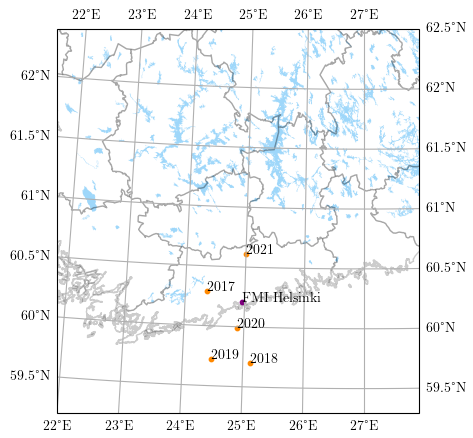
\includegraphics[width=\textwidth]{pics/geolocationmap2}
         \caption{Geolocation estimations for FMI Helsinki dataset.}
         \label{fig_geolocationhelsinki}
     \end{subfigure}
     \hfill
     \begin{subfigure}[b]{0.45\textwidth}
         \centering
         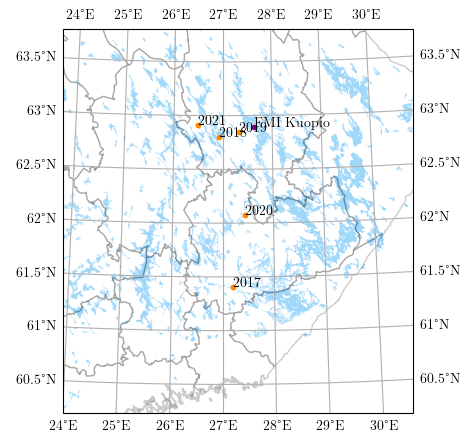
\includegraphics[width=\textwidth]{pics/geolocationmap3}
         \caption{Geolocation estimations for FMI Kuopio dataset.}
         
         \label{fig_geolocationkuopio}
     \end{subfigure}
     \hfill
     \label{fig_anglespace}
\end{figure}

In the Helsinki predictions figure, the estimated geolocations are scattered around the known installation location, showing very little bias and some random noise. Similar behavior can be seen in Kuopio predictions where two outliers 2017 and 2020 deviate more significatly. One degree on the latidue axis is approximately 110 km regardless of latitude and longitude, one degree of longitude is 56km at $60^\circ$ N and 50 km at $63^\circ$ N. As the deviation is strogest on the latitude axis, it is likely that the latitude prediction algorithm is more sensitive to variations in the data and further development should be focused on more accurate latitude prediction and day range selection.

\chapter{Estimating panel angles}
Solar panel installation angles are a large factor in deciding the energy output of a PV system. If panel angles can be freely chosen during planning and installation phases, it can make sense to either optimize for total power generation or power generation during peak consumption hours. This means that even if installation angles could be freely chosen, installation angles are unlikely to be the same for every system in the same geographical region. Panel angles may also be restricted by installation sites and mounting types.

% Panel racks have to be installed based on the available area 

%Installation type also plays a factor in choosing the panel angles. Panel angles may be restricted by 

 %In so called flush rooftop installations, the panels are installed to run along the roof and so the angles can not be freely chosen. Panels can also be rack mounted and these racks tend to be installed and oriented based on the available area as is the case with \ref{fig_fmikumpula_panels}. Due to the forementioned reasons, panel angles vary from installation to installation.

Panel angles can be difficult to measure accurately. The tilt angle of the panels or the angle between the panel normal and zenith(the point directly above) can easily be measured with an angle ruler and a bubble level, but the azimuth angle of the panels is much harder to measure with the same degree of accuracy. If an accurate compass is used and the difference between the magnetic north and the geographic north is taken into account, metal structures and electrical systems nearby can still distort local magnetic fields enough to cause errors in measurements. The challenges in taking accurate measurements are not insurmountable, but they may contribute to the inaccuracies and the lack of available information in PV installation parameter metadata. 

The space of possible panel installation angles can be thought as a half unit sphere in a spherical coordinate system where each point on the surface represents a direction to which the normal of the solar panels could be directed towards. A visualization of parameter space in 3D and 2D is shown in \ref{fig_halfdome} and \ref{fig_anglespace1}. The 3 dots in the subfigure b) mark the zenit for which azimuth is not well defined(red), the installation angles of FMI Helsinki installation azimuth $135^\circ$ tilt $15^\circ$(blue) and a close to power generation maximized installation with directly south facing panels with the tilt of $45^\circ$(black).


\begin{figure}[h]
	
     \centering
     \begin{subfigure}[b]{0.35\textwidth}
         \centering
         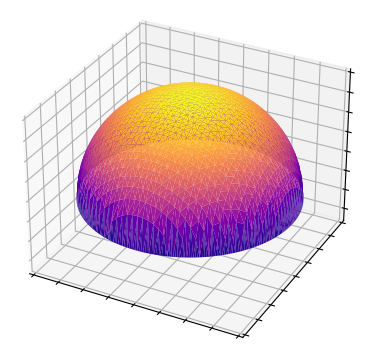
\includegraphics[width=\textwidth]{pics/halfdome}
         \caption{The space of possible angles as a 3D half sphere surface. Each point represents a possible tilt and azimuth combination.}
         \label{fig_halfdome}
     \end{subfigure}
     \hfill
     \begin{subfigure}[b]{0.35\textwidth}
         \centering
         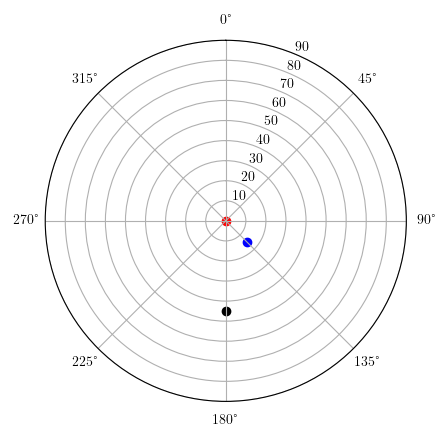
\includegraphics[width=\textwidth]{pics/polarplot}
         \caption{2D projection of the angle space, distance from center denotes the tilt angle of the panels and angle marks the azimuth.}
         
         \label{fig_anglespace1}
     \end{subfigure}
     \hfill
     \caption{Angle space visualizations.}
     \label{fig_anglespace}
\end{figure}


\noindent Estimating panel installation angles requires the use of multiple functions, each of which can be defined in multiple ways. These functions are defined in the following sections.
\begin{itemize}
  \item Prediction error function for quantifying how good a prediction was when the correct panel parameters are known.
  \item Model error function for measuring the error between simulated power values and measured power values.
  \item Multiplier matching function for matching the magnitude of simulated power values with the magnitude of measurements. This does not change the shape of simulations.
  \item Angle space discretization function for discretizing the angle space into $n$ discrete points which can then be tested with model error function.
\end{itemize}




\section{Prediction error function}
%The first part in developing a panel installation estimation algorithm is creating a metric for measuring how well the algorithm performs. 
In this thesis, the proposed error estimation method combines the tilt and azimuth delta values into one error angle value, the angular distance between two points on a spherical surface. The goal is then to develop a panel angle estimation function which achieves the lowest angle error value with the available datasets.

Alternative approaches can also be chosen as the function or functions for measuring the distance between two points in angle space can be defined in multiple ways. The simplest way is to use the delta of known tilt and azimuth angles as two separate error values without normalizing in any way. This method was used in Hagdadi's 2017 article but such values are not direcly comparable between installations as the significance of azimuth delta depends on tilt angle.

%Measuring the distance between two coordinate pairs in angle space is more complicated than measuring errors in latitudinal or longitudinal degrees. This difficulty rises from how the azimuth angle lines converge at the pole, resulting in a coordinate system where azimuth delta values are disconnected from the phenomena which they are trying to describe. If the tilt angle is near zero, azimuth delta becomes meaningless but at high tilt angles, even small azimuth delta values can be significant. If this is not corrected for, using azimuth and tilt deltas (changes in angles) as algorithm performance metrics would incorrectly suggest that the data quality of low tilt installations is lower than that of high tilt installations, or that the system is less capable of estimating the parameters of low tilt installations. Due to these reasons, a better way of measuring the distance between two points is needed, luckily the center angle between two points on an unit sphere is easy to solve with geometry and the resulting equation is rather simple.

%While there are no issues with using angles to denote the direction of the panels, the angle values do not map the possible panel angles into the angle space in a way which would make measuring the difference between two angle space coordinates easy. The issues rises from how the azimuth angle lines converge at the pole, resulting in a coordinate system where azimuth delta values are disconnected from the phenomena which they are trying to describe. For example, a 45 degree azimuth delta is fairly significant at tilt of 90 degrees but almost insignificant at 15 degree tilt. If this is not corrected for, using azimuth and tilt deltas (changes in angles) as algorithm performance metrics would incorrectly suggest that the data quality of low tilt installations is lower than that of high tilt installations, or that the system is less capable of estimating the parameters of low tilt installations. Due to these reasons, a better way of measuring the distance between two points is needed, luckily the center angle between two points on an unit sphere is easy to solve with some geometry and the resulting equation is rather simple.

\vspace{3mm}
\noindent\textbf{Deriving angle space distance equation}

\noindent Let $v= [v_1, v_2]$ and $k = [k_1, k_2]$ be two component angle-space vectors so that $v_1$, $k_1$ $\in$ $[0,90]$ and $v_2$, $k_2$ $\in [0,360]$. These vectors represent points on the surface of a unit sphere and their components are the angles of spherical coordinate system. The cartesian coordinates of these points are:
	\begin{align}
	x_v &= sin(v_1)cos(v_2)\\
	y_v &= sin(v_1)sin(v_2)\\
	z_v &= cos(v_1)
  \end{align}
  And
  \begin{align}
	x_k &= sin(v_1)cos(v_2)\\
	y_k &= sin(v_1)sin(v_2)\\
	z_k &= cos(v_1)
  \end{align}
\noindent And the cartesian distance between these two points can be calculated with the following equation:
\begin{align}
	d = \sqrt{(x_v-x_k)^2 + (y_v-y_k)^2+(z_v-z_k)^2}
\end{align}


\noindent The two points and the origin form an isoceles triangle with the sides from the origin to the vector end points having the length of 1 while the distance between the vector end points is the same as d.

\noindent As the lengths of three sides are known, the angles of the triangle can be calculated with the cosine rule. 
\begin{align}
	a^2 &= b^2 + c^2 - 2bc \cos(A)
\end{align}
Where
\begin{conditions}
 a     &  Side opposing the angle A, same as earlier value d \\
 b     &  Side opposing angle B, value is 1  \\   
 c	   &  Side opposing angle C, value is 1
\end{conditions}
\noindent Substituting known values into the cosine equation.

\begin{align}
	a^2 &= b^2 + c^2 - 2bc \cos(A)\\
	d^2 &= 1^2 + 1^2 - 2 \cos(A) \\
	d^2 &= 2 - 2 \cos(A)
\end{align}

\noindent Solving for angle A
\begin{align}
	d^2 &= 2-2\cos(A)\\
	2 \cos(A) &= 2 -d^2 \\
	\cos(A) &= \frac{2-d^2}{2} \\
	A &= \cos^{-1}(\frac{2-d^2}{2})
\end{align}

\noindent Renaming $A$ as $Error$.

\begin{align}
	Error &= \cos^{-1}(\frac{2-d^2}{2}) \label{errorangle}
\end{align}


\noindent By first calculating the distance between the vectors using equations 5.1-5.7 and then substituting the distance into equation 5.16, the resulting angle can then be used as an error value between two panel angle measurements. Python code based on this proof is included in appedix \ref{angular_distace_appendix}.


% This error value is the same as the angle between two points on the surface of a sphere. %In addition, if the deviation occurs only on the tilt axis, the error value and the tilt error are the same.% This makes the error values intuitive.
%In some ways, this method of calculating an error angle is analogous to moving the two angle vectors so that one of them aligns with the 0 tilt point and computing the tilt delta between the two points. Because of this, the error values are fairly intuitive and the error value should better represent the actual difference between installations than other error values calculated via other means.


\vspace{5mm}

%\section{Angle estimation error functions}
%The process of angle estimation requires the use of error estimation functions. The first function is needed for testing the accuracy of the algorithm by translating the known installation angles and the estimated angles into a meaningful error value. This is nontrivial as moving by a set angle value on the tilt and azimuth axis in spherical coordinate space result in different cartesian distances depending on the starting point. 


%The second function or set of functions is needed for evaluating how well a simulated irradiance curve fits the measurement data. Functions of this type can be used for parameter estimation by testing out possible parameter combinations and and choosing the combination which results in the lowest error between the simulated and measured values.


\newpage
\section{Simulation error function}
\label{section_simulation_error_function}
Simulation error function measures how much the predicted power generation values vary from the measured power generation values. The purpose of the simulation error function is to be able to generate a single numerical value which describes how well a certain parameter combination models the measurements. By then testing out multiple parameter combinations, the combination with the lowest simulation error function value should be the best fit and the parameters used for the simulation should be within a small error of the physical parameters of the solar PV installation. In \ref{fig_error} the error between a cloud free day and randomly chosen set of wrong simulation parameters is visualized.



\begin{figure}[h]
\centering
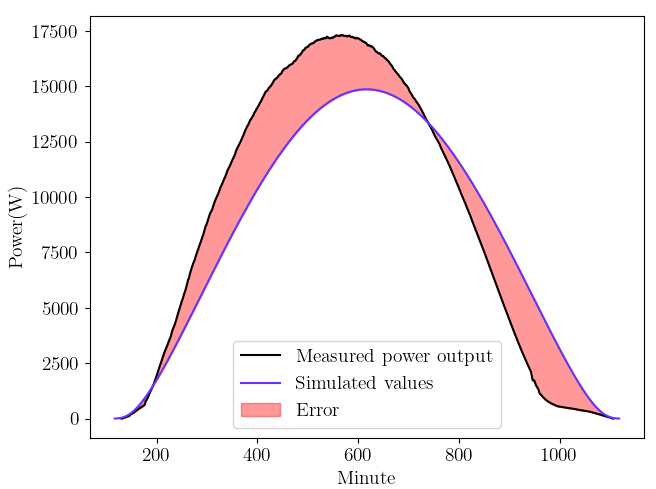
\includegraphics[width=0.6\linewidth]{pics/error}
\figcaption{Error area between measured power values and simulated irradiance values with different panel installation angles.}
\label{fig_error}
\end{figure}



\newpage
\subsection{Area based error function}
%\noindent \textbf{Area based error function}
The following function can be used in order to get a numerical value which signifies the area between simulated and measured power values. 

\begin{align}
	Error =  \Sigma_{t=0}^{1439} |m(t)-p(t)| \label{areaerror}
\end{align}

\noindent Where $m(t)$ is the measured power at minute $t$ and $p(t)$ is simulated power at minute $t$.

\vspace{5mm}
\noindent The error values can also be normalized so that the error value reflects the average percentual deviation between the measured and modeled values for each minute.

\begin{align}
	Error\_per\_minute =  \frac{\Sigma_{t=a}^{b} m(t)/p(t)}{b-a} \label{areaerrorpercents}
\end{align}

\noindent Where $m(t)$ is the measured power at minute $t$ and $p(t)$ is simulated power at minute $t$.

\subsection{Alternative simulation error functions}
\noindent Other error estimation methods could be used as well. Skew values, peak power generation minutes and other similar charasteristics could be measured and matched. The benefit of such charasteristics matching based error algorithms is that charasteristics errors have a direction as well as magnitude and these could be used in order to estimate the proximity and direction of the best fit in angle space. 

The downsides of using charasteristics are that measurement data contains noise which can distort the estimated values of charasteristics and having a direction and a magnitude is of limited value unless additional functions are created for turning these error values into directions in parameter space. These relationships between traits, their error directions and magnitudes could prove to be difficult to solve.


% Examples of some of the possible charasteristics can be seen in \ref{fig_charasteristics}.

\begin{figure}[h]
\centering
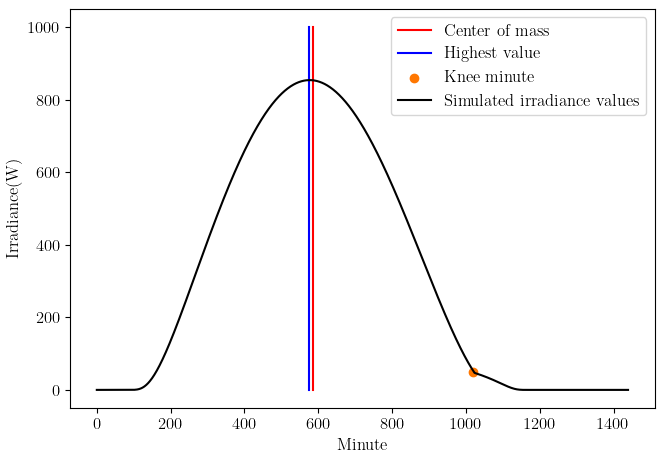
\includegraphics[width=0.5\linewidth]{pics/poa_charasteristics}
\figcaption{Center of mass, highest value and knee minute marked on a simulated irradiance figure.}
\label{fig_charasteristics}
\end{figure}




\newpage
\section{Multiplier matching}
As the plane of array irradiance model models the solar radiation towards a virtual 1 m$^2$ sized panel, using the values to simulate the power generation of a solar power installation requires the use of a multiplier. This multiplier is related to the efficiency and the surface area of the solar PV installation.

%holds information on the surface area and the efficiency of the solar panel installation. %For example, a 1 m$^2$ installation with the efficiency of 15\% would have the multiplier of 0.15 while as a 10 m$^2$ installation with the same efficiency would require the multiplier value to be 1.5. Thus the relationship between multiplier, efficiency and surface area is multiplier = efficiency*area.

%The multiplier value can be necessary for installation angle solving depending on the methods used, luckily solving the multiplier value can be almost trivial.

\subsection{Area based multiplier matching}
The multiplier value can be solved by making the assumption that a plane of array irradiance curve $p(t)$ with correct simulation parameters matches the measurements curve $m(t)$ in its shape but not magnitude. By calculating the sum of simulated and measured power values, their ratio can then be used as a multiplier. After scaling $p(t)$ with a multiplier to match $m(t)$ the two curves should be nearly inditinquishable. 
%This matching can be done by taking sums of measured and simulated irradiance and power values over a day and generating a ratio based on these sums. Thus, multiplier can be defined as follows:

\begin{align} 
	M_{multiplier} =  \frac{\Sigma_{t=0}^{1439} m(t)}{\Sigma_{t=0}^{1439} p(t)}\label{function_multipliermatch}
\end{align}

%And if the two curves do not match in shape, multiplying the simulated values by a constant should not change this fact as the ratio between measurements $m(t_0)$ and any other measurement $m(t_1)$ stays the same when both are multiplied by a non-zero multiplier. While this means that the multiplier variable can not be solved separately from panel installation angles, the multiplier can still be estimated each time a new set of parameters is evaluated. As the multiplier estimation method relies on the computation of two sums, the operation is computationally fast.

\begin{figure}[h]
\centering
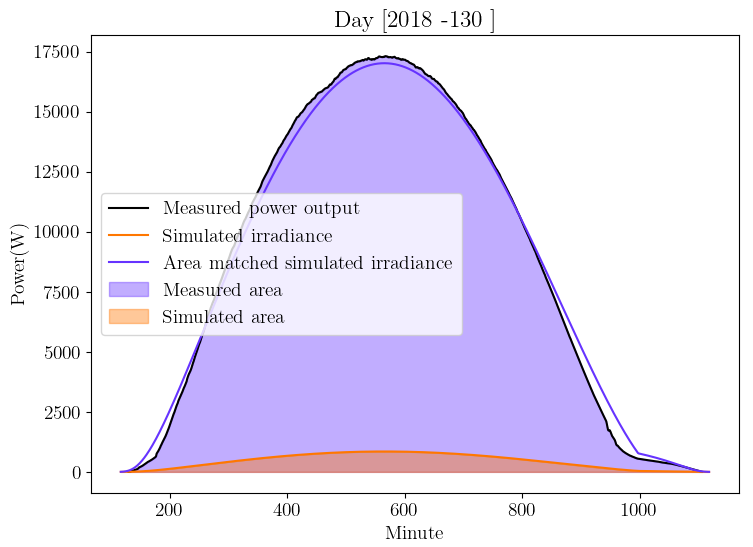
\includegraphics[width=0.6\linewidth]{pics/areamatching2}
\figcaption{Visualization of automated multiplier matching. Measurement data from FMI Helsinki dataset, plane of array irradiance simulation was computed with FMI Kumpula coordinates and installation angle parameters.}
\label{fig_area_match}
\end{figure}


\newpage

\subsection{Segmented multiplier matching}


\noindent The earlier multiplier matching method falls apart if the measurements used for multiplier solving contain deviations caused by clouds, trees or other sources. If the energy production during a certain section of the day varies from the expected, then this abnormal segment will affect the resulting multiplier value. If these deviating segments could be avoided, then partially cloudy days could still be used for multiplier matching. The process of segmentation can be done with multiple different methods. Here the inverval between the first and the last non-zero power minute of the day was split into 10 segments of equivalent length.



%day into multiple segments and then using the area matching algorithm on each of these segments to compute multiple multiplier values. If these multiplier values contain a tight cluster, then the average of this cluster can be used to approximate the correct multiplier value.

\begin{figure}[h]
\centering
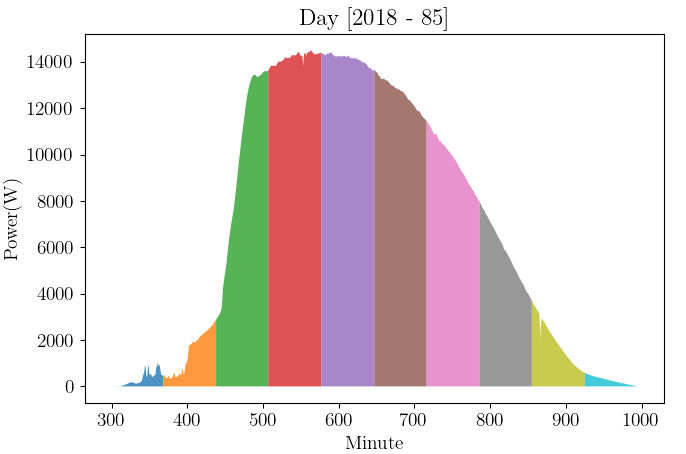
\includegraphics[width=0.8\linewidth]{pics/10segmentcloudy}
\figcaption{Partially cloudy day split into 10 segments.}
\label{fig_segment_match_segments}
\end{figure}


\noindent Now that the data is split into segments, the earlier area based multiplier algorithm can be used to compute a multiplier value for each segment. A mathematical representation for the segments $S_i$ multiplier $M_i$ could be as follows. 

\begin{align}
	M_i =  \frac{\Sigma_{t=a_i}^{b_i} m(t)}{\Sigma_{t=a_i}^{b_i} p(t)}
\end{align}

\noindent Where $a_i$ and $b_i$ are the first and last minutes of the interval \textit{i}.



\begin{table}[!ht]
\centering
\begin{tabular}{c|c} \hline

Interval & Multiplier\\
\hline
$[299, 367]$ & 1.26 \\
$[368, 437]$ & 3.22 \\
$[438, 506]$ & 16.56 \\
$[507, 576]$ & 21.68 \\
$[577, 646]$ & 21.58 \\
$[647, 715]$ & 21.52 \\
$[716, 785]$ & 21.23 \\
$[786, 854]$ & 19.80 \\
$[855, 924]$ & 16.08 \\
$[925, 994]$ & 16.80 \\
\hline\hline
\end{tabular}
\tabcaption{Segment based multiplier matching intervals and resulting multipliers. FMI Kumpula dataset day [2018 - 85] was used with irradiance simulation parameters listed in \ref{table_fmi_helsinki_kuopio_parameters}.}
\label{table_segmentmatch1}
\end{table}

\vspace{10mm}

\noindent In \ref{table_segmentmatch1} the segments 4 to 7 are all tightly grouped and their average is 21.50. These closely grouped segments, commonly referred to as clusters in the field of data science, can be identified algorithmically by locating a window that encompasses a relatively high number of values within it. For example a $\pm 5\%$ window $[M_i*0.95, M_i*1.05]$ would contain the cluster if any of the 4 cluster values was used as as $M_i$.

A possible issue with the clustering algorithm could rise from random chance. The last multiplier values 16.08 and 16.80 are close enough to the early 16.56 that due to random variation in the data, the algorithm could in some cases choose the wrong multiplier value cluster. The low values are unexpected as the plot appears to be free from cloud interference and it is possible that the deviation from the expected values occurs due to increased reflectivity of the solar panels resulting from a higher angle of incidence. This issue could be midigated to some extent by using a more advanced solar power generation simulation algorithm.


% High reflectivity is especially difficult to account for in this stage as the panel angles are not yet known.


%Regarding the observation that the last two segments result lower multiplier values than expected, despite the plot appearing to be smooth and interference free

%absence of apparent cloud interference in the plot, one possible explanation could be attributed to increased reflectivity of the solar panels resulting from a higher angle of incidence. High reflectivity is especially difficult to account for in this stage as the panel angles are not yet known.

% In figure \ref{fig_segment_match_segments} the same segments, marked in red to pink, can be seen to be well-behaving. The lower than expected multipliers for segments 1 to 3 are to be expected, but the deviance of segments 8 to 10 is somewhat unintuitive. One explanation could be higher reflectivity of the solar panels caused by the higher angle of incidence.




\begin{figure}[h]
\centering
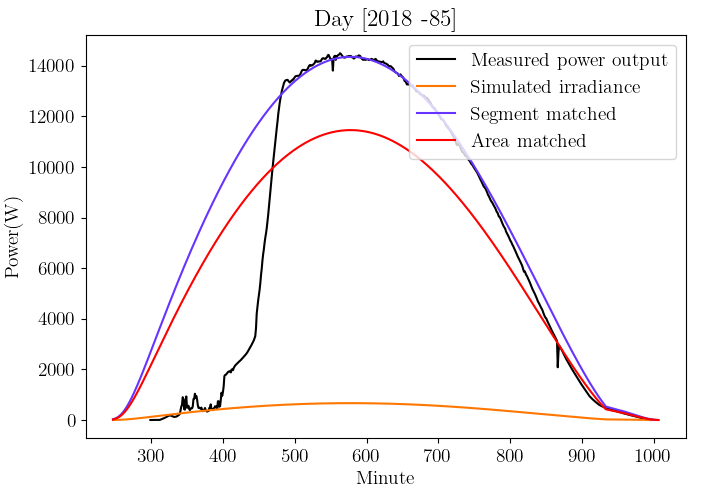
\includegraphics[width=0.8\linewidth]{pics/segmentmatch1}
\figcaption{Comparison of area and segmented area based multiplier matching algorithms on a partially cloudy day.}
\label{fig_segment_match}
\end{figure}


%This can be seen in figure \ref{fig_segment_match} where a day from FMI Kumpula dataset is plotted against an area matched irraidance simulation. Here the low power generation during early minutes of the day results in an underestimated multiplier.

%If this lower than normal power generation segment of the day could be algorithmically detected and avoided, the previously shown area matching algorithm would still allow the simulated curve to be matched with the non-cloudy section of the data. 



%The table \ref{table_segmentmatch1} shows 10 different segments and their corresponding multiplier values when area matching algorithm is applied to them. In the ideal case, all of these multiplier values would be identical, but due to shading in the early hours of the day, the first multiplier values are much lower than they would be for a clear day. The important values in this table are the tightly grouped multipliers 21.69, 21.57, 21.55 and 21.30. Their average 21.52 was used for the segment matched purple line in \ref{fig_segment_match} and at least in this case, the segment matched curve follows the measurements closely through most of the day. 

%This cluster of values can be detected algorithmically by taking each multiplier value $M_i$ and counting how many other values on the multiplier list fit with within the range of [$M_i - \delta $, $M_i + \delta $]. The more values that fit in this interval, the more likely those values are to perform well as the fitting multiplier. Delta value of 1 was used for figure \ref{fig_segment_match}. The clustering method and the delta values were arbitrarily chosen and so further experimentation with different clustering methods and delta values is recommended if such algorithms are applied to other datasets. For example, proportional instead of absolute ranges such as [$M_i (1- \delta) $, $M_i(1+\delta) $] may perform better when PV installations have differing power output ratings.


%Methods similar to the segment multiplier matching algorithm detailed in this section could be used for detecting cloudy time periods or shading.






\newpage

\subsection{Translating multiplier values to PV system rated power values}
As the simulated irradiance values are an estimation of power radiated towards a sigle square meter sized imaginary panel, the scaling multiplier can be used for estimating the power rating of a solar PV installation. The power ratings of PV installations describe the expected power generation in watts that could be expected to be generated during peak power generation hours if the panels were oriented optimally.

With the help of the rated power value, the surface area of the panels can be estimated. The precise estimation is difficult as different panel types and panel age affect the efficiency of PV systems, but having some frame of reference for installation sizes could prove to be useful in other studies where lidar data or satellite images are available.

\noindent \textbf{Rated power estimation equation}
\begin{align}
	RatedPower =  MP \label{ratedpower}
\end{align}
Where $M$ is the multiplier required to match the POA simulated values with measured values and $P$ is an estimation for solar irradiance per square meter or approximately 1000w. 

\vspace{5mm}
%The equation is as simple as it is because the plane of array irradiance simulations used for estimating the multiplier value already take the power generation losses due to different panel installation angles into account. 
\noindent By using \ref{ratedpower} and the clustered multiplier values from \ref{table_segmentmatch1}, the power rating of the Helsinki installation would be estimated as 21.5KW which is within close proximity the reported 21KW in \ref{table_fmi_helsinki_kuopio_parameters}.





\noindent \textbf{Panel area estimation equation}
\begin{align}
	PanelArea =  RatePower * \frac{1m^2}{\eta}
\end{align}
Where $\eta$ is the efficiency of solar panels, typically in the range of 0.15 to 0.20. The efficiency coefficient varies according to panel type, age, variance in manufacturing and other factors.
\vspace{5mm}

\newpage
\section{Angle space discretization}\label{angle_space_discretization}
The next step is angle space discretization. The panel angles are denoted with a doublet of tilt and azimuth values, ranging from 0 to 90 and 0 to 360 respectively. If the tilt and azimuth axes are discretized individually in steps of 5 so that tilt is [0, 5, 10, 15... 90] and azimuth [0, 5, 10, 15... 355], the permuations of these tilt and azimuth values create an even grid in the euclidean projection of angle space where x = tilt, y = azimuth. However as the physical phenomena represented by the angle values is not a point on a plane but a point on a half-sphere surface, this results in an uneven discretization \ref{fig_5step}. A better option is to use Fibonacci lattice \cite{fibolat2} for a more even distribution of points on a spherical surface \ref{fig_fibolat}.

%or another algorithm for a more even distribution of points on a spherical surface \ref{fig_fibolat}.

\noindent \textbf{Fibonacci lattice point n of k equation}
\begin{align}
	s &= n + 0.5 \\
	\phi &= acos(1 - 2 s / k) \\
	\theta &= \pi s (1 + \sqrt{5})
\end{align}
Where $n$ is the point number, $k$ is the amount of points, $\phi$ is the panel tilt angle and $\theta$ is the azimuth angle.
\begin{align}
	x &= cos(\theta)sin(\phi)\\
	y &= sin(\theta)sin(\phi)\\
	z &= cos(\phi)
\end{align}
$x$, $y$ and $z$ are the corresponding cartesian coordinates.
\vspace{5mm}


\begin{figure}
     \centering
     \begin{subfigure}[b]{0.45\textwidth}
         \centering
         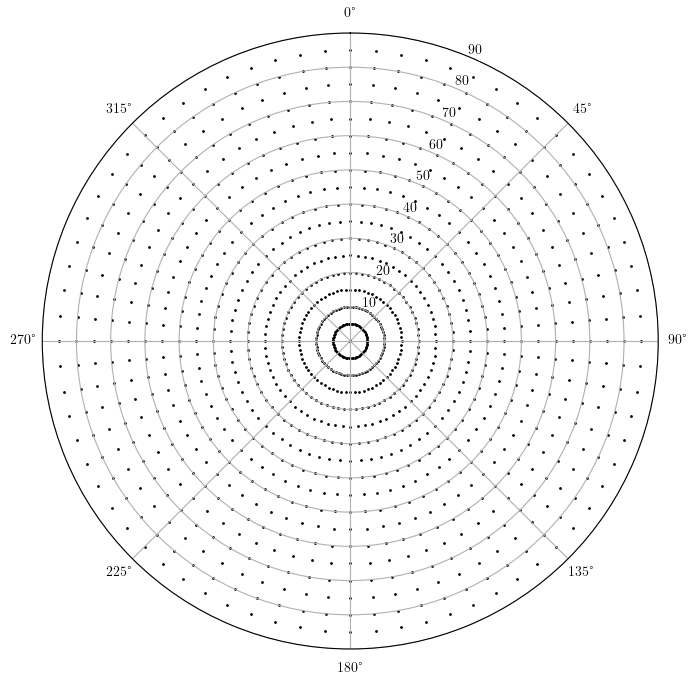
\includegraphics[width=\textwidth]{pics/disc5}
         \caption{In steps of 5 discretization with 1296 points}
         \label{fig_5step}
     \end{subfigure}
     \hfill
     \begin{subfigure}[b]{0.45\textwidth}
         \centering
         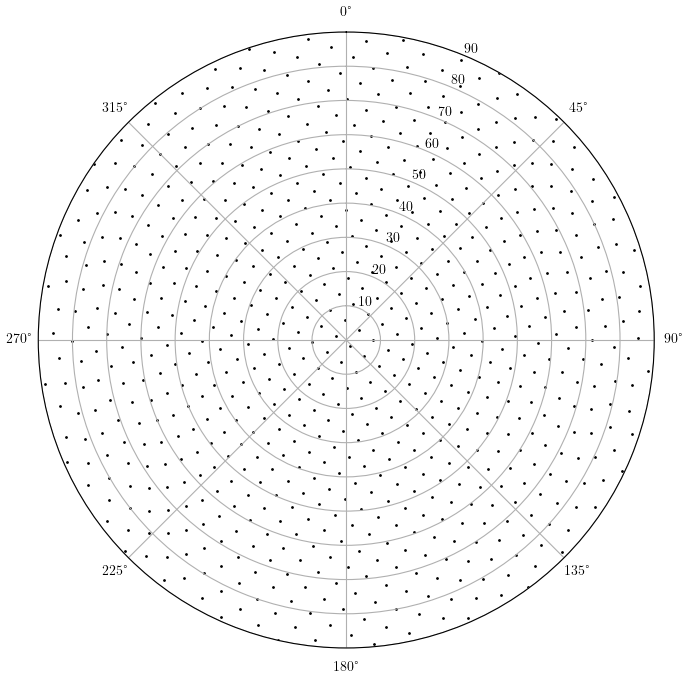
\includegraphics[width=\textwidth]{pics/fibolat1}
         \caption{Fibonacci lattice-based discretization with 756 points.}
         \label{fig_fibolat}
     \end{subfigure}
     \hfill
     
\caption{Comparison of two different discretization patterns. Fibonacci lattice based discretization on right shows a more even distribution of points than the latitude-longitude lattice. The minimum density is approximately the same in both graphs despite the difference in point counts.}
     \label{fig_5stepfibolat}
\end{figure}

\subsection{Importance of lattice density}\label{ss_lattice_density}
The density of lattices is an important measurable charasteristic which proves useful during the optimization of angle estimation algorithm. The most useful metric would be the sphere center angle distance between neighboring points. This would be useful as it can be used for determining whether errors in predictions are lattice or function fitting related. For example, if the lattice neighbors are approximately 1 degree away from oneanother and the predicted angle is 5 degrees off from the known installation angle, then the error is caused by model fitting and not lattice density as there must have been multiple lattice points closer to the known angle point than the discovered best fit. However if grid density is near to or lower than angle estimation error, the lattice is likely to be a contriburing to angle estimation errors.

Calculating neighborign center angle distances for both \textit{in-steps-of-n} and Fibonacci lattices is somewhat challenging. In \textit{in-steps-of-n}, the value \textit{n} can be used as an estimate for max center angle distance as \textit{n} will always be the tilt distance to the nearest neighbor with different tilt angle. With Fibonacci lattices the easiest way of estimating center angle distances is taking the coordinates of the first two lattice points and calculating their center angle distance with earlier error equation \ref{errorangle}. These first two points should be used as Fibonacci lattice points are distributed on a single arm spiral pattern, resulting in later sequential points being further from one another.

Another method for calculating Fibonacci lattice point distances is dividing the surface area of the angle space by the amount of calculated lattice points. This area-per-point value could then be used in order to estimate how far points are from oneanother on average. In later sections, the first two points derived distance will be used.

\newpage
\section{Solving panel angles}
Now that the geographic location and multiplier value of installation are known to be solvable and error functions have been defined, the last step is to solve the panel installation angles. The chosen method relies on splitting angle space into $n$ discrete points and evaluatin each of their fitness by calculating an error value. Here the angle space was split into 10 discrete points with fibonacci lattice \ref{angle_space_discretization} and the fitness of each point was evaluated with area error \ref{areaerror} and multiplier matching \ref{function_multipliermatch} functions. %The tilt-azimuth pair with the lowest error value was 31 



\begin{figure}[h]
\begin{floatrow}
\ffigbox{%
  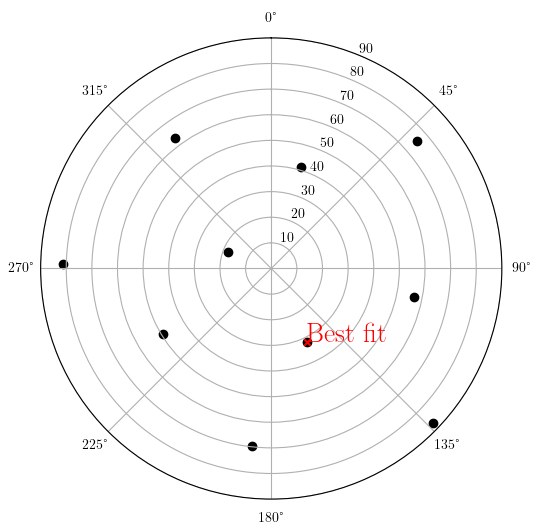
\includegraphics[width=1\linewidth]{pics/polarplot10}
  
  
}{%
\label{fig_polar10}
  \caption{Polar plot of test points for a single day of data from FMI Kumpula dataset.}%
}
\capbtabbox{%
  \begin{tabular}{c|c|c} \hline

Tilt & Azimuth & Error\\
\hline
18.19 & 291.25 & 3785693.23\\
\textbf{31.79} & \textbf{153.74} & \textbf{265843.23}\\
41.41 & 16.23 & 4331163.39\\
49.46 & 238.72 & 4861757.21\\
56.63 & 101.22 & 3811371.79\\
63.26 & 323.71 & 7196389.58\\
69.51 & 186.2 & 1795822.66\\
75.52 & 48.69 & 5985516.23\\
81.37 & 271.18 & 7403298.37\\
87.13 & 133.68 & 2957569.38\\
\hline\hline
\end{tabular}
}{%
  \caption{Tilt, azimuth and error table for single day.}
}
\end{floatrow}
\end{figure}


\noindent Now that the method can be seen to work, it is time to improve the results. This can be done by generating larger lattices and thus by evaluating higher amount of datapoints, the algorithm has a higher chance of finding the global minimum error point. As per \ref{ss_lattice_density}, Fibonacci lattice of 1000 points would have the angular resolution of approximately 4 degrees where as 10000 points would be near to 1.5 degrees. The performance can also be improved by evaluating best fits for multiple days at once. The resulting point cloud of best fits can then be used for averaging out noise in the predictions.

The plot \ref{fig_polar_multiyear} is a result of using the angle finding algorithm on 41 days from FMI Kumpula dataset with a Fibonacci lattice of 1000 points. The two darker spots near the center of the graph are the two most common best fits, [17.0$^\circ$, 138.4$^\circ$] with 17 and [22.7$^\circ$, 143.1$^\circ$] with 16 out of 41 days. These groupings are as close to the known installation angles of [15$^\circ$,  135$^\circ$] as could be expected from a 1000 point lattice. The next step is tightening the cluster, this can be done by adjusting the smoothness requirement of the cloud free day algorithm or by restricting the day range. In \ref{fig_polar_multiyear_summer} the tightening was accomplished with day range restrictions and 22 days were accepted by the algorithm.


%In \ref{fig_polarplot_13days} the polar plot is a result of taking the 13 best days from FMI Kumpula dataset year 2018 and using a fibonacci lattice with 500 test points. The most common best fit was [27.5$^\circ$, 150.8$^\circ$] with 5 occurances followed by [24.1$^\circ$, 138.4$^\circ$] with 4 days. These values are close to the 

\begin{figure}[h]
\begin{floatrow}
\ffigbox{
  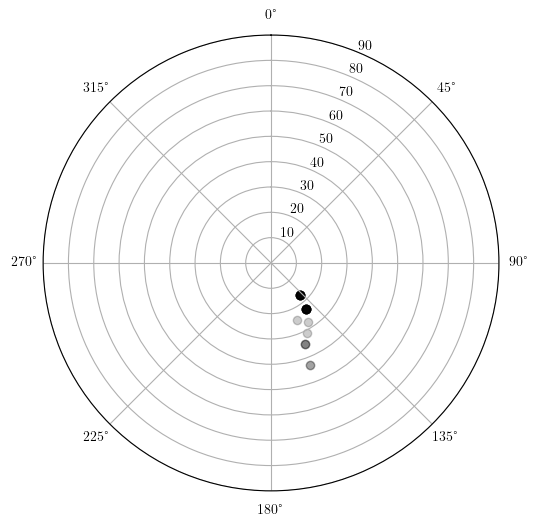
\includegraphics[width=0.95\linewidth]{pics/scatter_multiyear}
}{
  \caption{Best fits for multiple cloud free days from FMI Kumpula dataset.}
  \label{fig_polar_multiyear}
}
\ffigbox{%
 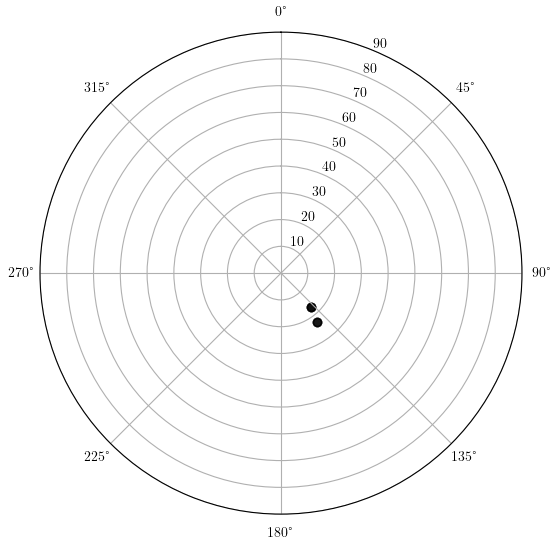
\includegraphics[width=0.95\linewidth]{pics/scatter_multiyear_summer}
}{%
\caption{Best fits when day range is restricted to days 140-220.}
  \label{fig_polar_multiyear_summer}
 
}
\end{floatrow}
\end{figure}

As all of the estimates converge on two neighboring points, the final step is increasing the lattice resolution further. With 10 000 point lattice, the cluster tightened further \ref{fig_polar_multiyear_helsinki10k}. Out of the 22 days, 7/22 or 32\% had best fit at [19.34, 136.87] with error of 4.38 degrees and 6/22 or 27\% at [17.74, 135.06] with error of 2.74 degrees. Rest of the best fits were distributed in smaller clusters near these points. The lowest angle distance best fit was [17.09, 130.32] with angle distance of 2.46 degrees. As the angle distance errors are higher than the discretization resolution and as the predicted angles are systematically biased, it would seem that the error is caused by the solar irradiance model or model fitting and not angle space discretization.


%As the angle distance errors are higher than the discretization resolution and as the results seem biased, the errors of the estimation algorithm would seem to be caused by inaccuracies in model fitting and not angle space discretization.



\begin{figure}[h]
\begin{floatrow}
\ffigbox{
  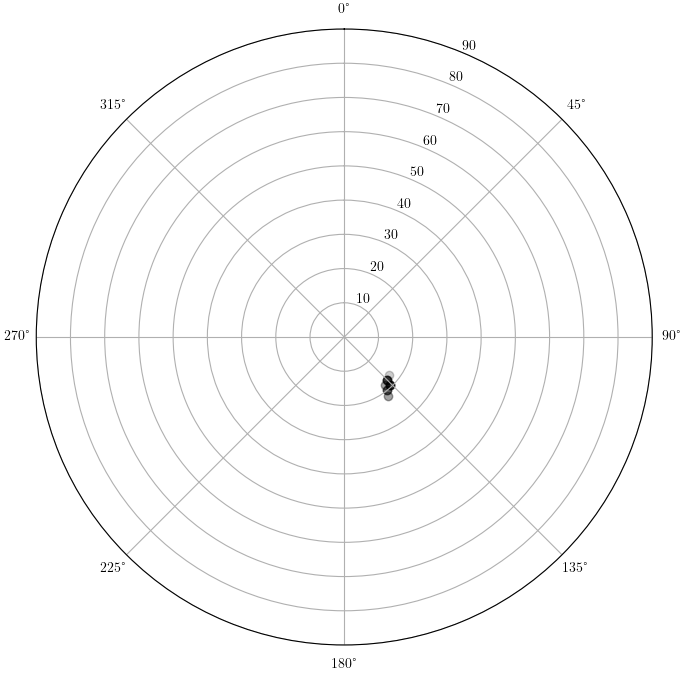
\includegraphics[width=0.95\linewidth]{pics/10khelsinki}
}{
  \caption{Best fits with 10 000 sample Fibonacci lattice and 22 days from FMI Kumpula dataset. Multiple years were used, day range restricted to 140-220. Actual installation angles were 15 degrees tilt, 135 azimuth.}
  \label{fig_polar_multiyear_helsinki10k}
}
\ffigbox{%
 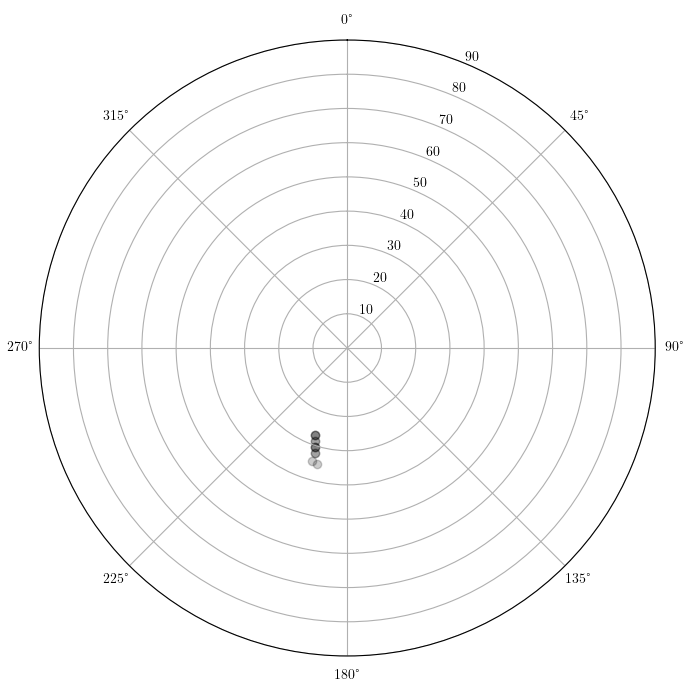
\includegraphics[width=0.95\linewidth]{pics/kuopio10kfitsplot}
}{%
\caption{10 000 sample Fibonacci lattice and 16 days from FMI Kuopio dataset. Multiple years were used, day range restricted to 140-220. Actual installation angles were 15 degrees tilt, 217 azimuth.}
  \label{kuopio10kfitsplot}
}
\end{floatrow}
\end{figure}


%\begin{figure}[h]
%\centering
%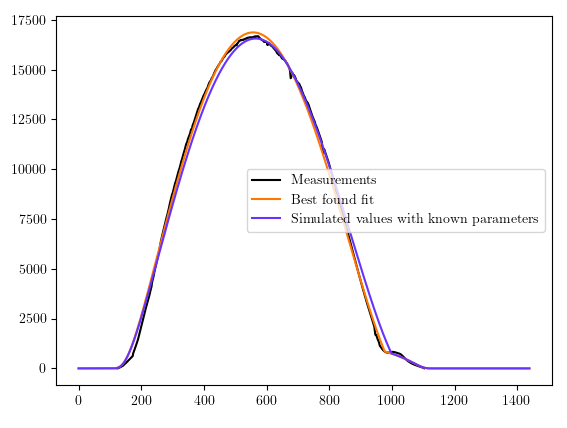
\includegraphics[width=0.8\linewidth]{pics/10kfitshelsinkiplot}
%\caption{Comparison between measured values, simulated values with known installation parameters and best found fit.}
%\label{fig_10kfitshelsinkiplot}
%\end{figure}



%day 141 predicted 17.74 135.06 delta degrees: 2.74 x
%day 145 predicted 19.92 141.6 delta degrees: 5.3
%day 148 predicted 19.34 136.87 delta degrees: 4.38 	x
%day 179 predicted 17.74 135.06 delta degrees: 2.74 x
%day 197 predicted 21.37 143.41 delta degrees: 6.87 y
%day 198 predicted 18.37 139.79 delta degrees: 3.64
%day 199 predicted 19.34 136.87 delta degrees: 4.38		x
%day 157 predicted 19.92 141.6 delta degrees: 5.3
%day 169 predicted 18.37 139.79 delta degrees: 3.64
%day 202 predicted 17.74 135.06 delta degrees: 2.74 x
%day 208 predicted 21.37 143.41 delta degrees: 6.87 y
%day 143 predicted 19.34 136.87 delta degrees: 4.38		x
%day 155 predicted 19.92 141.6 delta degrees: 5.3
%day 164 predicted 19.92 141.6 delta degrees: 5.3
%day 166 predicted 17.74 135.06 delta degrees: 2.74 x
%day 171 predicted 19.34 136.87 delta degrees: 4.38		x
%day 174 predicted 17.09 130.32 delta degrees: 2.46
%day 175 predicted 17.74 135.06 delta degrees: 2.74 x
%day 177 predicted 17.74 135.06 delta degrees: 2.74 x
%day 178 predicted 19.34 136.87 delta degrees: 4.38		x
%day 179 predicted 19.34 136.87 delta degrees: 4.38		x
%day 200 predicted 19.34 136.87 delta degrees: 4.38		x



%day 145 predicted 32.09 196.89 delta degrees: 18.65 x
%day 192 predicted 30.5 198.01 delta degrees: 16.96 y
%day 199 predicted 30.5 198.01 delta degrees: 16.96 y
%day 210 predicted 34.52 197.58 delta degrees: 20.9 z
%day 212 predicted 32.09 196.89 delta degrees: 18.65 x
%day 213 predicted 35.07 194.65 delta degrees: 21.86 k
%day 167 predicted 27.07 200.24 delta degrees: 13.37 i
%day 143 predicted 30.5 198.01 delta degrees: 16.96 y
%day 144 predicted 28.83 199.13 delta degrees: 15.21 l
%day 145 predicted 28.83 199.13 delta degrees: 15.21 l
%day 162 predicted 27.07 200.24 delta degrees: 13.37 i 
%day 167 predicted 27.07 200.24 delta degrees: 13.37 i 


\newpage
\subsection{Evaluation of exhaustive search results}
The estimated installation angles installations are fairly good. A delta of less than $4.5^\circ$ as was achieved with FMI Kumpula is small enough to be a result of measurement or rounding error. The estimates for FMI Kuopio are off by more than 10 degrees which is less encouraging. As the reported angles for FMI Kuopio were $15^\circ$ and $217^\circ$, it would seem like the angle measurements were rounded to nearest degree. This would eliminate the reporting accuracy as a plausible cause for the estimation errors and thus either there has been a reporting error or that the installation angle estimation algorithms are not performing as well for FMI Kuopio dataset.


\begin{figure}[h]
\begin{floatrow}
\capbtabbox{%
  \begin{tabular}{r|c|c|c} \hline
\multicolumn{4}{c}{FMI Kumpula}\\
\hline
n & Tilt & Azimuth & Error\\
\hline
7 & $19.34^\circ$ & $136.87^\circ$ & $4.38^\circ$\\
6 & $17.74^\circ$ & $135.06^\circ$ & $2.74^\circ$\\
4 & $19.92^\circ$ & $141.60^\circ$ & $5.30^\circ$\\
2 & $21.37^\circ$ & $143.41^\circ$ & $6.87^\circ$\\
1 & $21.37^\circ$ & $143.41^\circ$ & $6.87^\circ$\\
1 & $17.09^\circ$ & $130.32^\circ$ & $2.46^\circ$\\

\hline\hline
\end{tabular}
}{%
  \caption{Estimation results table for FMI Kumpula.}
}
\capbtabbox{%
  \begin{tabular}{c|c|c|c} \hline
\multicolumn{4}{c}{FMI Kuopio}\\
\hline
n & Tilt & Azimuth & Error\\
\hline
3 & $27.07^\circ$ & $200.24^\circ$ & $13.37^\circ$\\
3 & $30.50^\circ$ & $198.01^\circ$ & $16.96^\circ$\\
2 & $28.83^\circ$ & $199.13^\circ$ & $15.21^\circ$\\
2 & $32.09^\circ$ & $196.89^\circ$ & $18.65^\circ$\\
1 & $34.52^\circ$ & $197.58^\circ$ & $20.90^\circ$\\
1 & $34.52^\circ$ & $197.58^\circ$ & $20.90^\circ$\\
1 & $35.07^\circ$ & $194.65^\circ$ & $21.86^\circ$\\


\hline\hline
\end{tabular}
}{%
  \caption{Estimation results table for FMI Kuopio.}
}
\end{floatrow}
\end{figure}


Figures \ref{10khelsinkiplot} and \ref{10kkuopioplot} shows that the models based on best found fits are better fits than simulations done with the known parameters. This is true for both Helsinki and Kuopio datasets. This would suggest that the model fitting works as intended and that either the model is inaccurate or there is an error in reported panel angles. The more likely cause of the two is the the solar irradiance model and for some undetermined reason the error of the model is more significant for the Kuopio installation. Possible causes could be related to lower sun angles resulting in higher reflective losses or shadowing during last production hours which would also explain the uneven structure visible in the last non-zero hours in \ref{10kkuopioplot}.



\begin{figure}[h]
\caption{Comparison between a single day of measurements and two simulations. One with known installation angles and one with best found fit. Day is from FMI Kumpula dataset with reported installation angles of $15^\circ$ and $135^\circ$ degrees. Best fit at $19.34^\circ$, $136.87^\circ$}
\centering
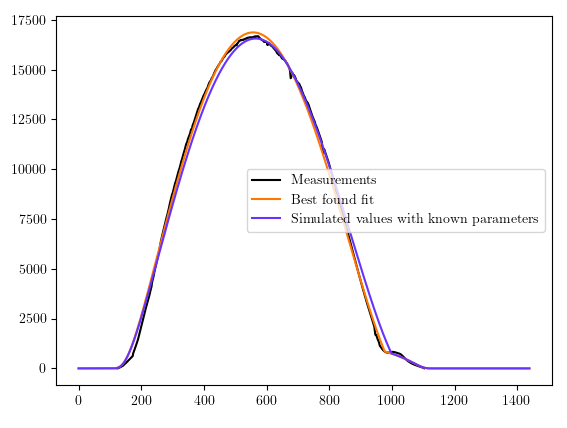
\includegraphics[width=0.6\textwidth]{pics/10kfitshelsinkiplot}
\label{10khelsinkiplot}
\end{figure}


\begin{figure}[h]
\caption{Comparison for FMI Kuopio installation. Panel angles are $15^\circ$ and $217^\circ$ degrees. Best found fit at $19.34^\circ$, $136.87^\circ$
}
\centering
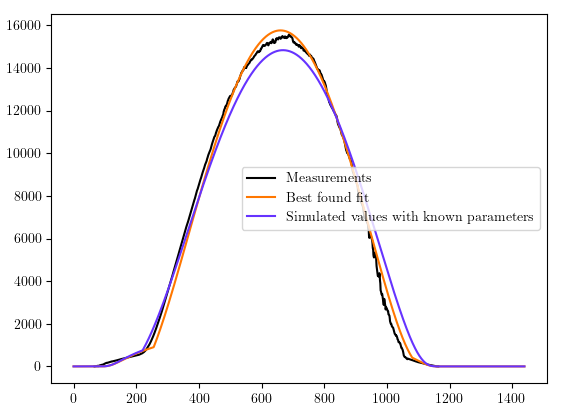
\includegraphics[width=0.6\textwidth]{pics/10kfitskuopioplots}
\label{10kkuopioplot}
\end{figure}


\section{Fast panel angle solving}
Solving panel angles by exhaustively testing 10 000 possible grid points takes up to an hour of computation time on the test system. This is not a limiting factor in research code, but exhaustive searches are inelegant compared to more intelligent approaches. Geometric intuition would suggest that the surface created by panel angle pairs and fitness values would resemble a downwards pointing cone-like shape where the best fit is the peak of the cone. If this is true, searching the whole angle space is not necessary as a gradient descent algorithm can be used to approximate the direction in which the best fit resides.

Whether the cone assumption is true can be visually examined by plotting the fitness values and observing the resulting heatmap. In \ref{fig_cone_shape}, the region where the global best fit resides is clearly the global minimum, but there appears to be a local minimum in the top part of the plot, near tilt $90^\circ$, azimuth $20^\circ$. Having more than one local minimum complicates efficient optimization but optimization is still feasible.


\begin{figure}[h]
\centering
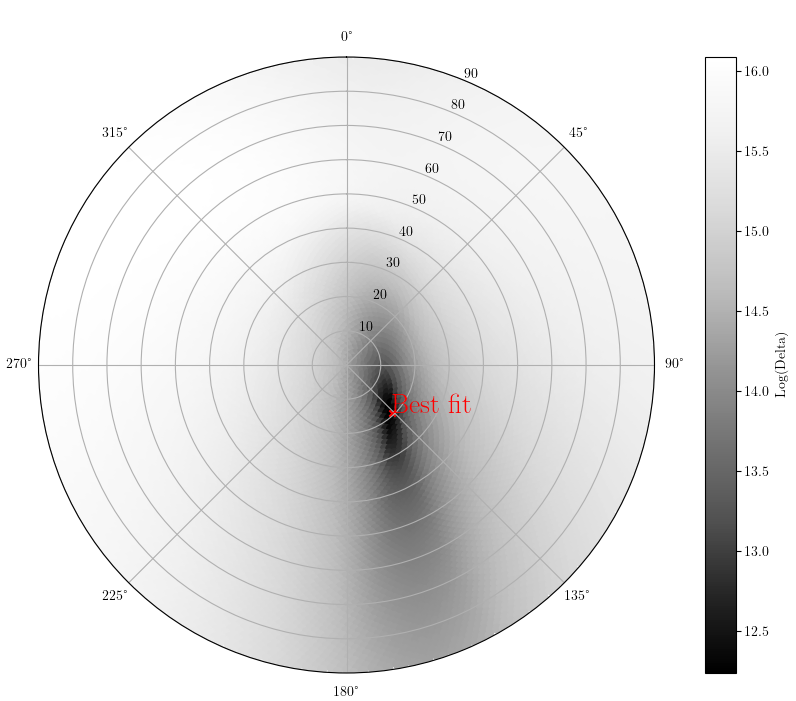
\includegraphics[width=0.6\linewidth]{pics/10kfitshelsinki}
\figcaption{Fitness heatmap.}
\label{fig_cone_shape}
\end{figure}

\subsection{Gradient search}
As the fitness surface is not defined by an easy to derivate multi parameter equation, directly solving for points where gradient reaches zero is challenging. However the gradient at a given point can still be numerically estimated and by taking steps in the direction of the gradient vector, local minimum can be found.

In x-y coordinate space, the numerical gradient for point 

\begin{align}
	\frac{\partial f}{\partial x}  &= f(p_1+x) - f(p_1)\\
	\frac{\partial f}{\partial y}  &= f(p_1+y) - f(p_1) \\
	\nabla f &= \begin{bmatrix}
	\frac{\frac{\partial f}{\partial x}}{\frac{\partial f}{\partial y}}
	\end{bmatrix} 
\end{align}

% \frac{\partial f}{\partial x} \end{bmatrix} 

% \nabla f &= \begin{bmatrix} \frac{\partial f}{\partial x \frac{\partial f}{\partial y}\end{bmatrix} 


\newpage
\subsection{Possible issues and further development ideas}

%Graphs \ref{fig_polar_multiyear_helsinki10kplot} and \ref{fig_polar_multiyear_kuopio10kplot} show that the found best fits are better fits for the data than simulations done with correct parameters. This would suggest that the model fitting and discretization both work as intended, but that the model being fitted does not work as intended. In general, the shape of the model becomes sharper when the panel tilt is near optimal in respect to sun elevation and broader when tilt deviates. This sharpening or broadening bears some reseblense to the error caused by not taking panel reflections into account and this could explain why predicted tilt angles are higher than reported installation angles. Developing a correction algorithm may be feasible, but replacing the plane of array irradiance model with a physically accurate solar power generation model is a better option.

%As the method shown earlier relies on model fitting, the accuracy of the model influences prediction accuracy. In general, the shape of the model becomes sharper when the panel tilt is near optimal in respect to sun elevation and broader when tilt deviates. This sharpening or broadening bears some reseblense to the error caused by not taking panel reflections into account and this could explain why predicted tilt angles are higher than reported installation angles. Developing a correction algorithm may be feasible, but replacing the plane of array irradiance model with a physically accurate solar power generation model is a better option.


The algorithm steps of cloud free day detection and lattice generation are computationally fast but evaluating a high density lattice for multiple days can take several minutes. For example, the time required for the generation of \ref{fig_polar_multiyear_summer} consist of 9 seconds of data loading and preprocessing, 1 second of cloud free day detection and 11 minutes of angle pair evaluation. With 22 days and 1000 points per day, the resulting 22 000 evaluations were done at the average speed of 33 evaluations per second. This comparably long processing time is due to inefficient code but the algorithms speed can also be improved by more intelligent latticing. The general location of the best fit could be solved with a low density lattice and a local high density lattice could then be used to estimate a higher accuracy angle pair. Combining code optimizations and localized angle space lattices could reduce the computation time significantly.






















\chapter{Conclusion}
The initial goal of this thesis was to find a simple way of estimating parameters of solar PV installations and this goal has been accomplished with moderate success. Some of the algorithms are thousands of lines of long, but the underlying mathematics was still kept simple. As a result, the code can be understood and modified by a wider audience. This is in particular contrast with AI and machine learning based approaches which often provide good results but which tend to be less insightful.

From the perspectives of mathematics and programming, model fitting problems are not particularly difficult. In this thesis, the challenges rose from optimization, understanding patterns in the data and discovering where the limits of the estimation algorithms come from. The insights gained while tackling these issues may be more valuable to other researchers than the final estimation algorithms. The most significant of which are the center angle error function, Fibonacci-lattice based angle space discretization and angle space resolution estimates. These were not mentioned in the cited literature and while the are most likely already used in other fields, they would most likely prove to be useful for similar studies conducted in the future.

While experimenting with the datasets, some interesting traits and phenomena were observed, some of which could warrant their own studies. For example, the figure \ref{10kkuopioplot} shows that the last hours of the specific day are noisy. This noise may play a significant role in the prediction erros and thus further studies in detection and classification of noise types in solar PV datsets would prove to be useful for all who perform analysis on solar PV installations. Perhaps the largest apparent obstacle in noise detection and classification studies is the temporal resolution as noise profiles of clouds, shadowing structures or temperature fluctuations may prove to be impossible to detect accurately at low temporal resolutions.

Lastly I would like to encourage other researchers to publish their research and code openly. During preminary research and literature reviews, the code examples or datasets which were used for research papers did not seem to be available. While research code may not be useful as is, 


 open research should be encouraged. During preminary research and literature reviews, there did not seem to be 

Lastly the state of open source research is somewhat concerning. Solar energy plays a significant role in green energy transition and 

\appendix
\section{Code samples}
The algorithms presented in this thesis are not very useful or easy to understand when presented with mathematical notations. The following listings contain code samples from github repository \cite{github_source} where the complete source code is published. 

\subsection{Cloud free day selection algorithm} \label{cloudfree_code}
% the \\ insures the section title is centered below the phrase: AppendixA

The three following code listings are used by the cloud free day selection algorithm. The first listing \_\_find\_smooth\_days() returns the list of day numbers and data from days which can be considered smooth. The second is a helper function used for calculating a normalized smoothness value for a given day with the help of Fourier transform based low pass filtering and the last listing is the FFT based low pass filter.

\begin{lstlisting}[language=Python, caption={Cloud free day finder main function}]

def __find_smooth_days(year_xa, day_start, day_end, threshold_percent):
    """
    :param year_xa: xarray of one year
    :param day_start: first day to consider
    :param day_end: last day to consider
    :param threshold_percent: smoothness percent, very best days for helsinki dataset have a smoothness value lower than 0.4. 1 seems to result in good values
    :return: list of xa days and a list of day numbers
    """

    # reading year from year_xa
    # if year_xa contains multiple years worth of data, the first will be chosen. Will most likely result in errors
    year = year_xa.year.values[0]

    smooth_days_xa = []
    smooth_days_numbers = []

    """
    The loop below goes through every day in given range from year of data
    If the range contains "bad days", this could cause issues. For example a day with zero power for every minute would be perfectly smooth, but at the same time it's the opposite of what we want
    """
    for day_number in range(day_start, day_end):
        day_xa = splitters.slice_xa(year_xa, year, year, day_number, day_number)

        smoothness_value = __day_smoothness_value(day_xa)

        
        if smoothness_value < threshold_percent:
            smooth_days_xa.append(day_xa)
            smooth_days_numbers.append(day_number)
        

    return smooth_days_xa, smooth_days_numbers
\end{lstlisting}

\begin{lstlisting}[language=Python, caption={Cloud free day day smoothness function}]
def __day_smoothness_value(day_xa):
    """
    :param day_xa: one day of real measurement data in xarray format, has to have fields minute and power
    :return:  percent value which tells how much longer the distance from point to point is compared to sine/cosine
    fitted curve. Values lower than 1 can be considered good. Returns infinity if too few values in day
    """

    # no values at all, returning infinity
    if len(day_xa["power"].values[0]) == 0:
        return math.inf

    day_xa = day_xa.dropna(dim="minute")

    # extracting x and y values
    minutes = day_xa["minute"].values
    powers = day_xa["power"].values[0][0]

    # too few values, returning inf
    if len(powers) < 10:
        return math.inf


    # transforming powers into fourier series and low pass filtering
    powers_from_fourier_clean = __fourier_filter(powers, 6)

    # this normalizes error in respect to value count, single value
    errors = abs(powers_from_fourier_clean - powers)
    errors_sum = sum(errors)
    errors_normalized = errors_sum / len(powers)

    # if max of powers is 0.0, then division by 0.0 raises errors. If we check max for 0.0 and return infinity
    # our other algorithm should disregard this day completely
    if max(powers) == 0.0:
        return math.inf
    # normalizing in respect to max value and turning into percents
    errors_normalized = (errors_normalized / max(powers)) * 100
    # this line may cause errors due to division max power 0.0

    return errors_normalized

\end{lstlisting}

\begin{lstlisting}[language=Python, caption={Cloud free day finder low pass filter}]

def __fourier_filter(values, values_from_ends):
    """
    :param values: array of values
    :param values_from_ends: how many of the longest frequencies to spare
    :return: values after shorter frequencies are removed
    """


    # FFT based low pass filter
    # Converting values to Fourier transform frequency representatives
    values_fft = numpy.fft.fft(values)
    # values in values_fft represent the frequencies which make up the values array. Structure is as follows:
    # [constant, low, low, ... med, med .... high, high .... med, med .... low,low]
    # this means that by zeroing out most of the values in the center, only the low frequency parts can be chosen.


    # zeroing out every value which is further than [values_from_ends] from the ends of the values_fft array
    values_fft[1+values_from_ends:len(values_fft) - values_from_ends] = [0] * (len(values_fft)-1 - 2 * values_from_ends)


    # reversing the fft operation, resulting in values with only low frequency components
    values_ifft = numpy.fft.ifft(values_fft)

    # ifft results can be partly imaginary, eq. 2.5 + 2i.
    values_ifft_real = []

    # saving only real components
    for var in values_ifft:
        values_ifft_real.append(var.real)

    # returning the result of the low pass filter

    return values_ifft_real
\end{lstlisting}


\subsection{Angular distance equation} \label{angular_distace_appendix}
This sample contains code used for computing the angular distance between two points on unit sphere surface. Used in panel installation angle error measurements.

\begin{lstlisting}[language=Python, caption={Angular distance function}]
def angular_distance_between_points(tilt1, azimuth1, tilt2, azimuth2):
    """
    Calculates the angular distance in degrees between two points on unit sphere surface.
    :param tilt1: point 1 tilt angle in degrees
    :param azimuth1: point 1 azimuth angle in degrees
    :param tilt2: point 2 tilt angle in degrees
    :param azimuth2: point 2 azimuth angle in degrees
    :return: sphere center angle between the two points
    """
    tilt1_rad = numpy.radians(tilt1)
    azimuth1_rad = numpy.radians(azimuth1)
    tilt2_rad = numpy.radians(tilt2)
    azimuth2_rad = numpy.radians(azimuth2)

    x1 = math.sin(tilt1_rad) * math.cos(azimuth1_rad)
    y1 = math.sin(tilt1_rad) * math.sin(azimuth1_rad)
    z1 = math.cos(tilt1_rad)

    x2 = math.sin(tilt2_rad) * math.cos(azimuth2_rad)
    y2 = math.sin(tilt2_rad) * math.sin(azimuth2_rad)
    z2 = math.cos(tilt2_rad)


    euclidean_distance = math.sqrt((x1 - x2) ** 2 + (y1 - y2) ** 2 + (z1 - z2) ** 2)

    center_angle = numpy.degrees(math.acos((2 - euclidean_distance ** 2) / 2))

    return center_angle
\end{lstlisting}
%
\renewcommand{\bibname}{References}  %  change References to Viitteet if writing in Finnish
%
\phantomsection
%
\addcontentsline{toc}{chapter}{\bibname}
\renewcommand{\baselinestretch}{1}
\label{bibbib}
\bibliography{example_refs.bib}
%
%\include{thesis_app} % If there are no appendices, remove this line.
%
\end{document}
